\documentclass{article}
\usepackage{lmodern}
\usepackage[fontsize=9pt]{scrextend}
\linespread{1.0}
\usepackage[english]{babel}
\usepackage[parfill]{parskip}
\usepackage{float}
\usepackage{hyperref}
\usepackage{multirow}
\usepackage{xcolor}
\usepackage{todonotes}
\usepackage{amsmath}
\usepackage{amssymb}
\usepackage{amsthm}
\usepackage{amsfonts}
\usepackage[margin=0.7in]{geometry}
\usepackage{array}
\usepackage{graphicx}
\usepackage{caption, subcaption}
\usepackage{enumitem}
\usepackage{graphicx}
\usepackage{tabularx}

\setlength{\parskip}{1em}

\makeatletter
\renewcommand{\rmdefault}{\sfdefault}
\def\subtitle#1{\gdef\@subtitle{#1}}

\def\leftHeader#1{\listadd\@leftHeader{#1}}
\def\rightHeader#1{\listadd\@rightHeader{#1}}

\def\@maketitle{
    \renewcommand{\do}[1]{##1

    }
    \begin{minipage}[t]{5cm}
        \flushleft
        \dolistloop{\@leftHeader}
    \end{minipage}
    \hfill
    \begin{minipage}[t]{5cm}
        \flushright
        \dolistloop{\@rightHeader}
    \end{minipage}
    \centering

    \vspace{1cm}
% \vfill
    {\huge\bfseries\@title\par}
% \vfill
    \vspace{0.75cm}
    \thispagestyle{empty}
}
\makeatother

\newcommand{\one}[1]{\colorbox{yellow}{$\displaystyle #1$}}
\newcommand{\two}[1]{\colorbox{green}{$\displaystyle #1$}}

\newcommand{\onen}[1]{\colorbox{yellow}{#1}}
\newcommand{\twon}[1]{\colorbox{green}{#1}}

\title{Reviewing and Extending Colorful Image Colourisation}
\leftHeader{Fabian Denoodt}
\leftHeader{Ward Gauderis}
\leftHeader{Pierre Vanvolsem}
\rightHeader{Deep Learning}
\rightHeader{Faculteit Wetenschappen}
\rightHeader{Vrije Universiteit Brussel}
\leftHeader{15/01/2023}

\begin{document}
\maketitle

\section{Introduction}

Automated image colourisation is the process of adding colours to grayscale images using computational means. This a challenging problem as it requires preserving the details and features of the original image, while also producing realistic colours. It is an inherently ambiguous and even subjective problem.
However, the field has recently seen significant improvements through the use of deep learning.\\
Images are usually represented in the RGB format, which consists of three channels, each channel corresponding to the amount of red, green, and blue an image contains. Each channel gets a value assigned and the three channels together form the colour of a pixel. Another way of representing a colour in a pixel is using the Lab colour space. In this format, the L channel represents the luminosity of the image, and the a and b channels, combined, represent the colour.\\
There have been multiple attempts to tackle the problem of image colourisation. In this work, we reproduce the deep image colouriser proposed by~\cite{colourful}. Unlike prior approaches, the authors propose treating the problem as a classification problem rather than a regression problem, which results in more vibrant colourisations. We focus on the colourisation of vehicles. Additionally, we introduce a simplified neural network architecture that is more adequate for the given dataset. As a result, we observe that the model generates more realistic colourisations of images on the vehicle dataset.

The tasks in the group project were divided as follows. Fabian and Pierre performed the literature review and the preparatory work of transforming the regression problem into a classification problem, such that Ward could train the models and evaluate the results. The preparatory work mainly consisted in defining the loss function, implementing functions for class rebalancing, and defining the necessary image transformation functions. Ward was mainly responsible for implementing the architectures, training the different models, and presenting the results. This same task division was adhered to when writing the report.

In what follows, we provide a discussion on the related work on image colourisation. We continue by describing more thoroughly the techniques proposed by \cite{colourful} and we specify how we dealt with concepts not specified in the paper. We move forward to describe the methods we used to implement and train our models and, finally, we conclude by discussing the experimental results and their interpretation.

\section{Literature Review}
Multiple approaches to colourise images using deep learning techniques have already been attempted. The first paper proposing this technique, called \textit{Deep Colorization}~\cite{deep} redefines the colourisation problem to be able to apply deep learning techniques. It also proposes a joint bilateral filtering-based post-processing step to ensure artefact-free quality and developed an adaptive image clustering technique to incorporate global image information. The authors of the paper conclude by discussing some limitations of their novel technique and by demonstrating plenty of experiments that outperform the up-to-that-point state-of-art algorithms both in terms of quality and speed for automatic colourisation.\\
This novel approach encouraged a lot of researchers to apply deep learning techniques to colourise images by improving the techniques for automatic colourising. Meanwhile, other researchers applied deep learning techniques to colourise images by giving more control to the user of the model. This can be done by allowing the user to colourise the images by adding colour strokes to a greyscale image. The model will then colourise the image based on the location and colour of the strokes. These methods are proposed by Kevin Frans~\cite{pierre1}. \\
Another user-guided image colourisation approach uses a colour palette to colour the original greyscale image. This technique was first explored by Huiwen Chang~\cite{pierre2}. A deviation of this approach uses a reference-coloured image to colour the original greyscale image by using the colours that are present in the reference-coloured image. This approach was first proposed by Lvmin Zhang et al.~\cite{pierre3}. More recently, language-based user-guided image colourisation approaches have been proposed. These techniques require a text description of how the user wants the greyscale image to be colourised. This method was proposed by Jianbo Chen~\cite{pierre4}.\\
The last paper we mention is the \textit{Colorful Image Colorization} paper \cite{colourful}. This paper proposes an automatic colourisation technique that colourises greyscale pictures with a plausible colourised version of the image. They address a problem most implementations of deep automatic colourisation have, namely desaturated colourisations. This is solved by using class rebalancing and using one of the first convolutional neural networks for colourisation. According to the authors, their approach results in state-of-the-art performance on several feature learning benchmarks. Due to the many advantages of their automated approach and its interesting reformulation of the colourisation task, we have decided to reproduce and build further on their work.

\section{Colourisation as Classification}
Consider we are given a grayscale input image $X$. This image can be represented as
$X\in\left[0..255\right]^{H \times W \times 1}$, 
where $W$ denotes the width and $H$ denotes the height. We wish to obtain the original colours of $X$. However, these colours must be represented in some form. We shall assume images to be in the Lab colour space. This means that each pixel of a Lab-image is a triplet $(L, a, b)$, where $L$ denotes the lightness and the channels $a$ and $b$ combined will specify the colour. So that predicting the $a$ and $b$ channels for each pixel corresponding to the grayscale image, suffices to obtain the coloured image. The input channel $L$ and predicted channels $a$ and $b$ can then be combined to obtain a fully coloured Lab-image. Our target predictions $Y$ are thus of the form $Y\in\left[0..255\right]^{H \times W \times 2}$.\\
This colourisation problem can thus be formally defined as finding the optimal function $\mathcal{F}$ in the equation below, where $\hat{Y}$ corresponds to the estimation of ground truth image $Y$:
\[\mathcal{F}\left(X\right)=\hat{Y}\]
One may then wonder how to quantify the quality of $\mathcal{F}$. The most evident measure may be to compute the distance between $Y$ and $\hat{Y}$ by computing the mean squared error $\ell(Y, \hat{Y}) = (Y - \hat{Y})^2$. However, notice how incorrect values
for $\hat{Y}$ that are close to the mean are less likely to be punished hard, compared to incorrect answers that are far from the
mean. It turns out that these colours, near the mean, are dark and greyish. Hence, optimizing $\mathcal{F}$ for the mean squared error loss will most likely lead to desaturated images.

\subsection{Regression to Classification}
Instead of treating the colourisation task as a regression problem, Zhang et al.~\cite{colourful} propose a different approach that handles it as a classification task, resulting in more accurate and diverse colourisations. The authors will no longer directly predict the $(a, b)$ pair for each pixel. Instead, given one pixel's $L$ value, the authors predict not the most likely $(a, b)$ pair, but the probability for every combination of $a$ and $b$ values for that pixel. Hence the colourisation task, which originally required finding the optimal $\mathcal{F}$, has now been transformed to optimize $\mathcal{G}$ in the following equation:
\[\mathcal{G}(X) = \hat{Z}\]
where $\hat{Z}\in\left[0,1\right]^{H\times W\times Q}$. $Q$ corresponds to the number of plausible $(a, b)$ pairs. Since the colour space is continuous, the set of $(a, b)$ tuples is infinitely large, however, we quantize the colour space into bins. We will later discuss how to go from the continuous $(a, b)$ space to a discrete finite space over $Q$. Figure~\ref{fig:conversion} displays the dimensions of $Y$ and $Z$ side by side. If we pay attention to the shape on the right side of the figure, we note that each pixel contains $Q$ values. Each such value refers to the probability for a specific $(a, b)$-tuple. Thus, each pixel ${\hat{Z}}_{h,w}$ corresponds to a probability density function (pdf). An example of such a pdf is shown in Figure~\ref{fig:density}.

\begin{figure}[h]
    \centering
    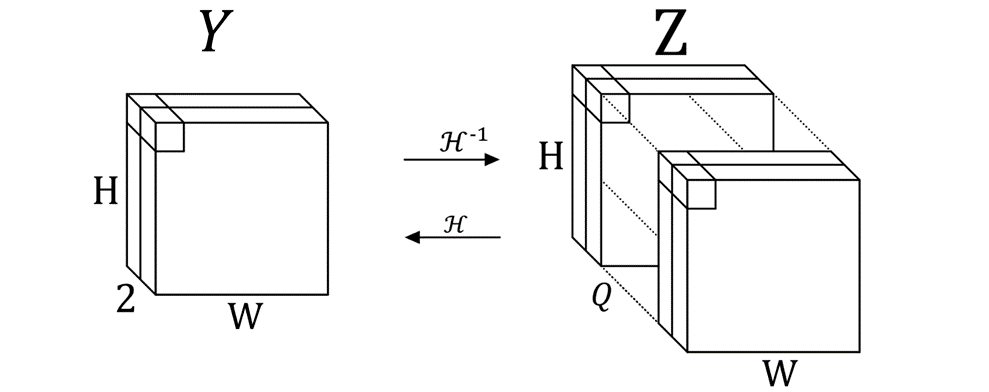
\includegraphics[width=0.6\textwidth]{GRAPHS/conversion.png}
    \caption{Visualisation of ground truth $Y$, intermediate ground truth $Z$ and their relationship via $\mathcal{H}$ and $\mathcal{H}^{-1}$ transformation functions; $Y$ contains two channels corresponding to the $(a, b)$ channels from the Lab colour representation. $Z$ contains $Q$ channels, such that each element in $Z_{h,w}$ is a $Q$-dimensional hot-encoded tuple of the form $\left(0,\ldots1,\ldots0\right)$, indicating the probability of each $(a, b)$ tuple. 
    }
    \label{fig:conversion}
\end{figure}

Given a grayscale image $X$, a probability density function is computed for each pixel, rather than the exact $\left(a,b\right)$ values of that pixel. Given such an estimation $\hat{Z}$, we would need its respective counterpart $\hat{Y}$ to be able to visualise the coloured image. This is done via the transformation function $\mathcal{H}$ which is defined as follows:
\[\mathcal{H}\left(\hat{Z}\right)=\hat{Y}\]
Zhang et al.~\cite{colourful} propose multiple implementations for $\mathcal{H}$. The straightforward technique for obtaining $\hat{Y}$ from $\hat{Z}$ is by selecting the $(a, b)$-tuple that corresponds to the highest probability in each pdf of $\hat{Z}$ (mode). This may lead to spatial inconsistencies. This means that certain pixels in the same neighbourhood might have very different colours, for example, some regions of a bus may be red and other regions blue. The opposite end of the spectrum to obtain ${\hat{Y}}_{h,w}$, is to compute the mean of the pdf and select the corresponding $(a, b)$ tuple. This will lead to spatially consistent, but desaturated results. Instead, the authors do not directly compute the mean on each pdf ${\hat{Z}}_{h,w}$, but will first adjust ${\hat{Z}}_{h,w}$ to have much stronger peaks. This will lead to a middle ground between desaturated images and spatial inconsistencies. The distributions ${\hat{Z}}_{h,w}$ are adjusted as follows:
\[{f_T(\hat{Z}}_{h,w})=\frac{\exp\left(\tfrac{log\left({\hat{Z}}_{h,w}\right)}{T}\right)}{\sum_q\exp\left(\tfrac{log\left({\hat{Z}}_{h,w,q}\right)}{T}\right)}\]
where $T$ is the temperature variable. Small values for $T$, e.g. $0.1$, will lead to the distribution $f_T(\hat{Z}_{h,w})$ having very large but thin peaks, while larger values, e.g. $1$, will lead to small peaks. Computing the mean of $f_T(\hat{Z}_{h,w})$ will lead to a single element of the distribution $\hat{Z}_{h,w}$, which corresponds to an $(a, b)$-pair.\\
We also define the inverse of $\mathcal{H}$, called $\mathcal{H}^{-1}$, as follows:
\[\mathcal{H}^{-1}\left(Y\right)=Z\]
The careful reader may have noticed how the hat symbol is no longer displayed in the equation above. This is because $\mathcal{H}^{-1}$ will be used to obtain $Z$, which will serve as the ground truth when evaluating the corresponding estimations $\hat{Z}$ in the loss function. In figure~\ref{fig:density}, two plausible pdfs are shown for a single pixel in $\hat{Z}$ and $Z$ respectively. The left image corresponds to a prediction of the mapping function $\mathcal{G}$, which was defined earlier. The right image corresponds to a distribution for a single pixel of the ground truth $\mathcal{H}^{-1}\left(Y\right)=Z$. Notice how the right figure is always $0$, except for one $(a, b)$-pair, because we use a one-hot encoding.

\begin{figure}[h]
    \centering
    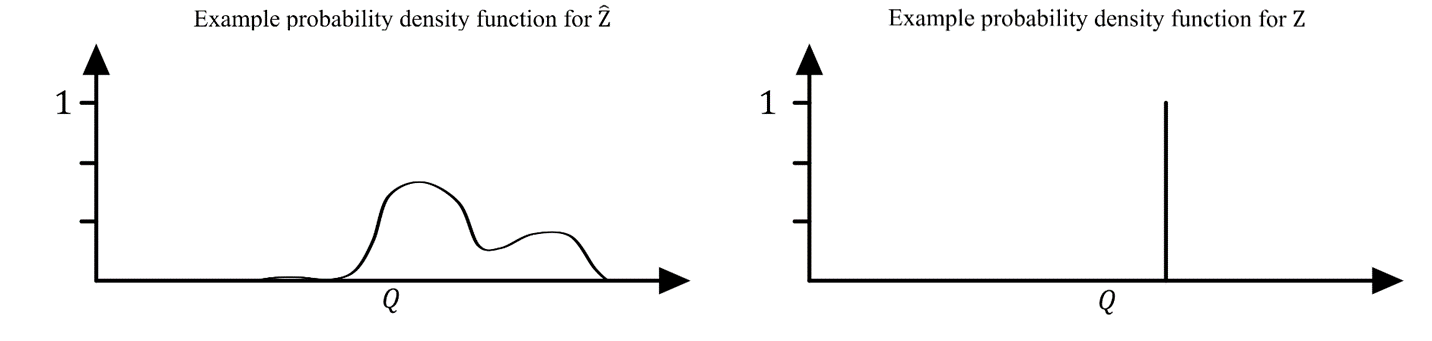
\includegraphics[width=0.9\textwidth]{GRAPHS/density.png}
    \caption{
        Visualisation of plausible distributions ${\hat{Z}}_{w,h}$ and $Z_{w,h}$; the distributions correspond to a single pixel of an image.}
    \label{fig:density}
\end{figure}

\subsection{Classification Loss}
We shall now discuss how to optimize $\mathcal{G}\left(X\right)=\hat{Z}$ to obtain vibrant colours. Consider the two distributions shown in figure~\ref{fig:density}. Our evaluation metric should obtain a small value when the two distributions are similar and a large value when the distributions strongly differ from each other. As we mentioned earlier, the colourisation task is transformed from a regression problem into a multiclass classification problem. We shall make use of the cross-entropy loss function. The estimation accuracy for a single distribution of a pixel ${\hat{Z}}_{h,w}$ can then be evaluated with respect to its ground truth counterpart $Z_{h,w}$ as follows: $\ell\left({\hat{Z}}_{h,w}, Z_{h,w}\right)=-\sum_q{[Z}_{h,w,q}\log({\hat{Z}}_{h,w,q})]$, where $q$ denotes each plausible $(a,\ b)$ combination. By computing this single metric for each pixel of the image, we obtain the following loss function:
\[\ell\left(\hat{Z},Z\right)=-\sum_{h,w}v(Z_{h,w})\sum_q[Z_{h,w,q}\log(Z_{h,w,q})]\]
where $v\left(\cdot\right)\in \mathbb{R}$ denotes the class rebalancing function. $v$ takes as input a pixel distribution $Z_{h,w}$. When class rebalancing is not active, this would be equivalent to $v\left(Z_{h,w}\right)=1$ for any $Z_{h,w}$. We will now discuss the class rebalancing function $v\left(\cdot\right)$ in more detail.

\subsection{Class Rebalancing}
As every colour does not appear equally often in the dataset, by classifying the $\left(a,b\right)$ values, certain classes will have more data points than others and our dataset will be imbalanced. Hence, frequently occurring colours will be more likely to be predicted by the model than rare colours. In the context of our dataset, which contains realistic images, dark colours such as grey and brown are more common than vibrant colours. To make the model more likely to also predict rarer vibrant colours, the authors will rebalance the loss for classes that do not contain a lot of data points at training time.\\
Consider the following, assume we are given two ground truth pixels, one pixel is a frequently occurring brown, and the second pixel is a rare pink. To make sure the model is also likely to make rare predictions, we want to punish it more severely when it inaccurately predicts the colour brown when it should be pink, compared to predicting pink when it should be brown. How severe the punishment must be, is quantified by the class rebalancing function $v\left(\ .\ \right)$. It is defined as follows:
\[v(Z_{h, w}) = w_{q^*} \quad \text{where} \quad q^* = \arg\max_q Z_{h, w, q}\]
Consider we have somehow computed the collection of weights $w$ for all the $Q$-values, which contains large values for rare colours and small values for frequently occurring colours. The equation $v\left(Z_{h,w}\right)=w_{q\ast}$ then implies that given a ground truth distribution $Z_{h,w}$, we select the weight in $w$ that corresponds to the ground truth $(a, b)$-value. This will be the result of $v\left(\cdot\right)$. Hence, since v$\left(\cdot\right)$ will contain large values greater than one for rare colours, the punishment for not predicting rare colours will be more severe in the loss function $\ell\left(\hat{Z},Z\right)$ defined above.\\
We will now discuss how to define $w$ such that it obeys these properties. The formal definition is described as follows:
\[w\propto\left(\left(1-\lambda\right)\widetilde{p}+\frac{\lambda}{Q}\right)^{-1},\quad\mathbb{E}\left[w\right]=\sum_q{\widetilde{p}}_qw_q=1\]
where $\widetilde{p}$ is the colour distribution of the entire dataset, $\lambda$ is a scaling factor equal to $0.5$, and $Q$ corresponds to the number of colour bins, equal to 313. $\widetilde{p}$ is smoothed with a Gaussian kernel of size $\sigma=5$. The weight distribution $w$ over the $Q$-values can then be computed practically, by first defining it as the right-hand side of the proportional equation above, and then normalizing it by dividing it by $\sum_q{\widetilde{p}}_qw_q$.

\subsection{Discretising an Infinite Colour Space}
We will now discuss the problem of quantizing the continuous $(a, b)$ colour space, into a one-dimensional discrete set of $Q$ elements. We define this problem as finding the mapping function $t:A\times B\rightarrow Q$, where $A\times B$ denotes the infinite amount of combinations of $(a, b)$-colour tuples. This mapping function is needed for translating $Y$ images into their respective counterpart $Z$, which is done in the function $\mathcal{H}^{-1}\left(Y\right)=Z$, which we discussed earlier.\\
The authors do not specify in much detail how to define this transformation function $t:A\times B\rightarrow Q$. We propose our own method instead. Consider that the Python library Scikit-Image already does part of the bin discretisation for us, since the values for $a$ and $b$ range between $a\in\left[-127,128\right]$ and $b\in\left[-128, 127\right]$. We further reduce this space to the ranges: $a\in\left[-12,12\right]$ and  $b\in\left[-12,12\right]$, by dividing values by $10$ and rounding downwards to an integer. Hence an $a=76$, would be transformed to $a=7$. Furthermore, since certain $(a, b)$ pairs within the given ranges do not exist, we define a mask based on the colour distribution of our dataset $\widetilde{p}$, which we also used in the image rebalancing equation. Based on this mask we can filter out $(a, b)$-tuples which do not exist within the dataset, further reducing the plausible set of $(a, b)$-tuples from $Q=\left|\left[-12,12\right]\right|\cdot\left|\left[-12,12\right]\right|=25\cdot=625$, to $Q=212$. If the plausible range of $(a,b)$-values is represented as a two-dimensional array, this array can then be flattened to a one-dimensional array, such that $t$ can be further specified from the respective indexes of that array.

The authors of the original paper propose a grid of $Q=313$ plausible $(a, b)$-bins and map each plausible $(a, b)$-pair in the colour space to the nearest bin in the grid. The exact details on how these values are computed are not specified, however, their $Q=313$ corresponds to the number of bins that are visible to the human eye, when assuming a grid of size $10$. Online, we have found the author's mapping file, which corresponds to the mapping function $t:A\times B\rightarrow Q$. To make sure our implementation gets as close to the original work as possible, we continued with the authors' grid discretisation implementation instead, making use of the grid of size $Q=313$.\\
Furthermore, when we look at the distribution displayed on the right of figure 2, we suggest that when computing a distribution $Z_{h,w}$, given a ground truth tuple $Y_{h,w}\in A\times B$, a one-hot encoding takes place. Indeed, the result is then the distribution with the single spike at the location that corresponds to the $(a, b)$-pair. However, during training the authors propose to apply a soft encoding instead. This means that the distribution will also include the four nearest neighbours of the correct $(a, b)$-pair. Finally, a Gaussian kernel is applied, resulting in a smoother distribution than shown in figure~\ref{fig:density}.

\section{Experimental setup and results}
In the following subsections, we discuss the experimental setup and methodology used to reproduce and build
on the work of~\cite{colourful} and the results we obtained.

\subsection{Network Architecture}
To predict a probability distribution over all 313 discretised $(a, b)$ values for every pixel in the input image,
based only on the lightness channel of that image, we employ a very deep convolutional neural network similar to
that proposed by~\cite{colourful}.\\
The network consists of 8 convolutional blocks, as shown in Figure~\ref{fig:network}.
Each block consists of 2 or 3 convolutional layers with ReLU activations, followed by batch normalisation.
Since no pooling layers are used, all downsampling or upsampling of spatial resolution
is achieved by strided or transposed convolutions.
This has the advantage that the network does not depend on a fixed image input resolution,
although, as discussed in the next subsection, we train and evaluate the models specifically for 256x256 images.
So it can be expected that the network might not perform as well on images of different resolutions.\\
In the internal convolutional blocks 5 and 6, the dilation is increased to 2, which allows the network to
keep the spacing at which neighbouring elements of the kernel are evaluated, relative to the input resolution,
constant, before eventually decreasing it again in consecutive blocks.
All details about the network architecture can be found in Table~\ref{tab:network}.
Models trained with this architecture have a total of 32\:235\:385 parameters.

\begin{figure}
    \centering
    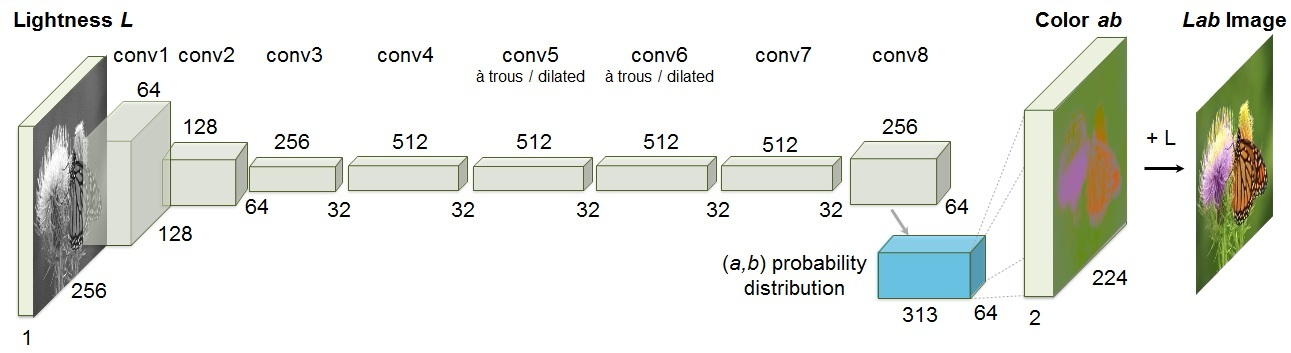
\includegraphics[width=0.9\textwidth]{net_diagram.jpg}
    \caption{Architecture of the network; image taken from the original paper \cite{colourful}}.
    \label{fig:network}
\end{figure}

\begin{table}
    \centering
    \begin{tabular}{|c|c|c|c|c|c|c|c|}
        \hline
        \textbf{Layer}        & \textbf{Resolution} & \textbf{Channels} & \textbf{Kernel size} & \textbf{Stride} & {\textbf{Dilation}} & \textbf{Normalisation} \\
        \hline
        \textbf{lightness}    & 256                 & 1                 & -                    & -               & -                   &                        \\ \hline
        \textbf{conv1\_1}     & 256                 & 64                & 3                    & 1               & 1                   & -                      \\
        \textbf{conv1\_2}     & 128                 & 64                & 3                    & 2               & 1                   & 1                      \\ \hline
        \textbf{conv2\_1}     & 128                 & 128               & 3                    & 1               & 1                   & -                      \\
        \textbf{conv2\_1}     & 64                  & 128               & 3                    & 2               & 1                   & 1                      \\ \hline
        \textbf{conv3\_1}     & 64                  & 256               & 3                    & 1               & 1                   & -                      \\
        \textbf{conv3\_2}     & 64                  & 256               & 3                    & 1               & 1                   & -                      \\
        \textbf{conv3\_3}     & 32                  & 256               & 3                    & 2               & 1                   & 1                      \\ \hline
        \textbf{conv4\_1}     & 32                  & 512               & 3                    & 1               & 1                   & -                      \\
        \textbf{conv4\_2}     & 32                  & 512               & 3                    & 1               & 1                   & -                      \\
        \textbf{conv4\_3}     & 32                  & 512               & 3                    & 1               & 1                   & 1                      \\ \hline
        \textbf{conv5\_1}     & 32                  & 512               & 3                    & 1               & 2                   & -                      \\
        \textbf{conv5\_2}     & 32                  & 512               & 3                    & 1               & 2                   & -                      \\
        \textbf{conv5\_3}     & 32                  & 512               & 3                    & 1               & 2                   & 1                      \\ \hline
        \textbf{conv6\_1}     & 32                  & 512               & 3                    & 1               & 2                   & -                      \\
        \textbf{conv6\_2}     & 32                  & 512               & 3                    & 1               & 2                   & -                      \\
        \textbf{conv6\_3}     & 32                  & 512               & 3                    & 1               & 2                   & 1                      \\ \hline
        \textbf{conv7\_1}     & 32                  & 256               & 3                    & 1               & 1                   & -                      \\
        \textbf{conv7\_2}     & 32                  & 256               & 3                    & 1               & 1                   & -                      \\
        \textbf{conv7\_3}     & 32                  & 256               & 3                    & 1               & 1                   & 1                      \\ \hline
        \textbf{conv8\_1}     & 64                  & 128               & 3                    & .5              & 1                   & -                      \\
        \textbf{conv8\_2}     & 64                  & 128               & 3                    & 1               & 1                   & -                      \\
        \textbf{conv8\_3}     & 64                  & 128               & 3                    & 1               & 1                   & -                      \\
        \hline
        \textbf{distribution} & 64                  & 313               & 1                    & 1               & 1                   & -                      \\
        \hline
    \end{tabular}
    \caption{Architecture of the network. Only convolutional layers are used in the network, making it
        independent of the input resolution of the image.}
    \label{tab:network}
\end{table}

Since such a large architecture requires a lot of memory and computation power, not to mention
the amount of training data required, we have also implemented a simplified network architecture.
This architecture keeps the same number of convolutional blocks, but reduces the maximum depth of the blocks
to 2 and limits the maximum number of channels to 416.
These modifications mainly impact the complexity of the internal hidden convolutional blocks 4, 5 and 6 while
preserving the overall design.\\
In this way, we can halve the number of parameters of the network, while almost doubling
the training speed, and preserving the same predictive performance.
Models created with this architecture have only 15\:387\:513 parameters.

\subsection{Dataset}
The network described in the original paper was trained on the ImageNet dataset \cite{imagenet} containing
more than 1.3 million images from 1000 different classes.
RGB images are converted to the Lab colourspace and from the lightness channel the model tries to predict
the chromatic $a$ and $b$ channels. The prediction is then compared to the true $a$ and $b$ values.\\
As per the recommendation of the teaching assistants, we have tried to balance the dataset size and the number of training epochs
in such a way that the training time on our available hardware takes approximately one hour while obtaining the
best possible fit without overfitting.
This allowed us to experiment with many different model configurations and to investigate the observations
of \cite{colourful} in more depth.

We have created two different datasets, subsets of the ImageNet dataset, which are both partitioned
into training, validation and testing sets with a random 80-10-10 split (with a fixed seed for reproducibility).
To avoid overfitting to these smaller training sets, the training images were augmented
by applying random horizontal flips and random crops of size 176x176.
The validation and testing sets were not augmented, but the images were cropped to 256x256 pixels for conformity.\\
Since it is impossible to achieve similar performance to the original paper on much smaller datasets,
we have decided to limit the scope of our models to the colourisation of grey images of vehicles.
This ensures that our models can focus only on the colourisation of images of a select
few classes within ImageNet and learn features specific to vehicles without overfitting.\\
The first \textit{experimental} dataset contains 2500 images of 5 classes: vehicles, aeroplanes, fishing boats, armoured cars and bumper cars.
We found that these classes have many similarities, while still being very distinct
in terms of colours. While, for example, most vehicles are photographed in urban environments with dense backgrounds,
aeroplanes are generally present in the sky and fishing boats on the water. Armoured cars, on the other hand, are usually
photographed in a natural environment while bumper cars always appear in very hectic brightly coloured carnival environments.
This dataset was used for training all experimental models.\\
The second \textit{final} dataset subsumes the first one and adds 5 more similar classes: boat racing, auto racing, racing, motorcycling,
and bicycling. With a total size of 5600 images, this set was used to further improve our two best-performing experimental models with
more data and more training epochs.

\subsection{Models and Training}
All models were created using the PyTorch framework \cite{pytorch}, with help of the
torchvision library for image transformations and the scikit-image library for
image processing.
The models were configured, trained, and evaluated and the results were visualised using a Jupyter
notebook, while the actual model and dataset code are organised in classes in separate files.
We provide one general configurable \texttt{Model} class from which the baseline and simplified
models inherit, as well as a \texttt{Dataset} class for loading and preprocessing the datasets.

In total, we have created 7 experimental models which were trained on the \textit{experimental} dataset
for 100 epochs with a batch size of 32. Per model,
this took about 2 hours on a single NVIDIA GeForce GTX 1060 6GB GPU and 1 hour on
the hardware offered by the Google Colab platform.\\
In addition, we have created 2 final models, based on the configuration of the most
promising experimental models, which were trained on the \textit{final} dataset for
as long as we could afford on our hardware at the time (7 hours and 24 hours respectively).\\
All models were trained from scratch, using the Adam optimizer with $\beta_1 = 0.9, \beta_2 = 0.99$,
an initial learning rate of $3.16 \cdot 10^{-5}$ and a weight decay of $10^{-3}$, similar to
the original paper.\\
Now follows a description of the models and their configurations in chronological order of the experiments.

\paragraph{\textit{Euclidean} model}
As a baseline, we created a regression model based on the original paper's architecture.
The only difference is that instead of predicting a distribution over the discretised $(a, b)$ colour space for every pixel,
we directly predict the $a$ and $b$ values. Because distances in the Lab colour space are
based on the perceptual distance between colours, this model employs the Euclidean distance, or
L2-norm, as a loss function. This model is expected to perform poorly because it will be encouraged to
predict the mean $a$ and $b$ values when
minimising this loss. The ab colourspace, however, is inherently multimodal and a wide range
of colours could be plausible for a pixel, given the lightness values.
For this reason, desaturated predictions are expected from the \textit{Euclidean} model.
\paragraph{\textit{Unbalanced one-hot} model}
Our first improvement on the baseline is a model that predicts a distribution over the discretised
$(a, b)$ colour space. We use the same discretisation as the original paper,
reducing the entire $(a, b)$ space to 313 possible $Q$-values visible to the human eye.
As this reduces the learning problem to classification, the model is trained using the cross-entropy loss function,
but without class rebalancing.
To encode the true $(a, b)$ values into a distribution over the $Q$-values, we use a one-hot encoding.
This combination means that the model is encouraged to predict the most common $Q$-value,
so we expected the predictions of this mode to be rather greyish as well.
\paragraph{\textit{Unbalanced} model}
We improve on the previous model with a more sophisticated encoding of the true $(a, b)$ values.
This model uses a soft encoding of the labels so the model can learn the relationship between the $Q$ classes quickly.
This is done by weighting the 5 $Q$-values nearest to the true $(a, b)$ value based on their distance, using
a Gaussian kernel with a standard deviation of 5.
The model is expected to better predict regions of smoothly varying colours, but still with quite desaturated colours
as pixels with low $(a, b)$ values are much more common in the dataset.
\paragraph{\textit{Rebalanced} model}
This is the original model used by \cite{colourful}.
The cross-entropy error at every pixel is reweighted based on the frequency of the true $Q$-value in the dataset.
Naturally, desaturated colours will occur more often. By assigning a higher weight to the loss of pixels with rare true $Q$-values,
the model is forced to prioritise predicting these rare colours as well.
This is a form of class rebalancing, which is often applied in classification problems with imbalanced datasets.
To calculate the weights for the loss of a pixel, we make use of the empirical frequency distribution of the $Q$-values
over the entire ImageNet dataset, as provided by \cite{colourful}.
With this modification, the predicted images should be more saturated, although some exotic colours might be overly present.
\paragraph{\textit{Rebalanced smoothed} model}
The original paper mentions that smoothing the empirical frequency distribution of the $Q$-values might improve the results further
by reducing the weighting difference between extremely rare and common $Q$-values. This model uses a rebalanced cross-entropy loss
weighted by values based on the empirical frequency distribution smoothed with a Gaussian kernel with a standard deviation of 5.
We could expect this modification to reduce overprediction of extremely rare colours, while still discouraging greyish predictions.
\paragraph{\textit{Rebalanced ours} model}
Since our models target only the colourisation of greyscale images of vehicles, using a frequency distribution of the $Q$-values specific
to this type of image can result in more accurate predictions. For example, one could expect that some saturated colours are very common
in vehicle photography, but might be rare in other types of images. By creating an empirical distribution over our training set
only, we update the relevance of the frequency information resulting in more specialised weights. In Figure~\ref{fig:distribution},
we compare the empirical distributions over the $Q$-values of the ImageNet dataset and its smoothed version to
our empirical distribution over the \textit{experimental} training set only.
It is clear that our distribution has more and sharper peaks than the ImageNet distribution because
the ImageNet dataset contains a much wider variety of images.
No model with a smoothed distribution, calculated only on the training data, was created as the original
\textit{Rebalanced smoothed} model did not perform better than the original \textit{Rebalanced} model (see next section).

\begin{figure}
    \centering
    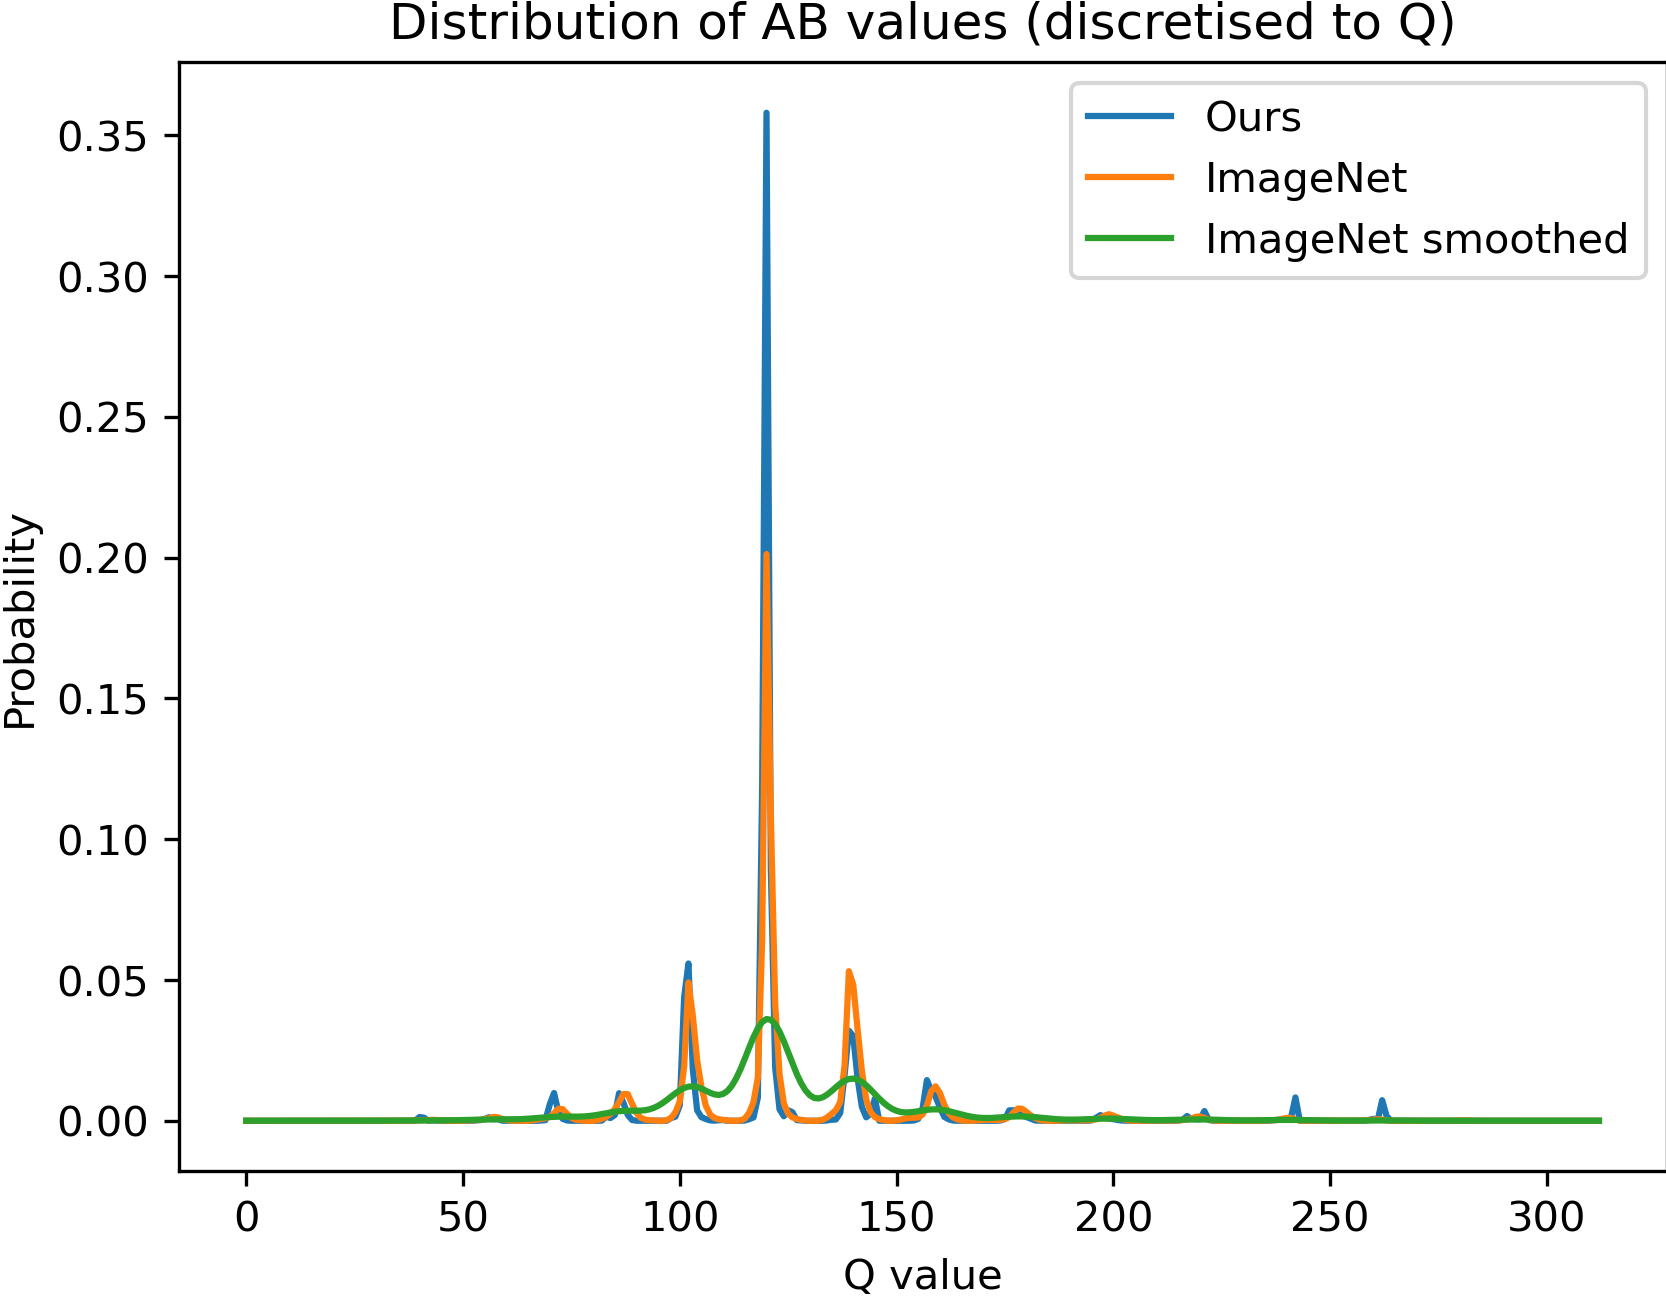
\includegraphics[width=0.5\textwidth]{GRAPHS/distribution.png}
    \caption{Empirical distributions over the $Q$-values, calculated in different ways}
    \label{fig:distribution}
\end{figure}

\paragraph{\textit{Simplified} model}
This model builds further on the \textit{rebalanced ours} model by using the previously discussed simplified architecture.
Since we are only training on a very specific subset of the ImageNet dataset, a complex architecture,
like the one discussed in \cite{colourful}, might be overkill and might even overfit the training data.
In addition, we observed that this complex architecture was very slow to train, both in terms of computation time
and in terms of the decrease in loss over epochs. This could potentially be attributed to the vanishing gradient problem
occurring in very deep networks.
The simplified architecture trains almost twice as fast and we could expect the model to update its fewer parameters more quickly,
leading to the loss decreasing faster, while still being able to capture the complexity of the vehicle colourisation problem.
\paragraph{\textit{Rebalanced ours final} model}
Observing the success of the \textit{Rebalanced ours} model, we decided to train a final model using the same architecture
and loss function, but on the larger \textit{final} dataset. We managed to train the model from scratch for 190 epochs in 7 hours.
\paragraph{\textit{Simplified final} model}
The \textit{Simplified final} model performed almost the same as the \textit{Rebalanced ours} model in the evaluation
but was much faster to train. Inspired by the lecture on transfer learning, we created the \textit{Simplified final} model
by finetuning the parameters of the \textit{Simplified} model on the \textit{final} dataset for an additional 500 epochs in 24 hours.

In Figure~\ref{fig:learning_curves}, we show the training and validation loss curves for the most
interesting experimental and final models. Many models use different loss functions,
so comparing the model performance based on absolute loss values is not very meaningful, but we
can still observe the general trend of the loss curves.
Notice that the scale of the x-axis of the bottom two graphs is much larger.\\
Looking at the training and validation loss of the \textit{Unbalanced} model,
we can see both drop very quickly in the first 20 epochs but then slow down considerably.
This is a general trend for all learning curves and by inspecting the intermediate saved
checkpoints, we can explain this behaviour.
All models start with a very high loss, which is caused by the initial random weights, but
very quickly they learn to predict the most common desaturated colours resulting in grey images.
It is actually in the flat tail of the learning curve that the models learn to predict
vibrant colours again and escape the 'grey' local minimum. These small reductions
in training loss result in perceptual changes in the predictions that are much larger to the human eye.\\
Compared to the learning curve of the \textit{Unbalanced} mode, the \textit{Rebalanced} model's
loss is quite a bit higher, rougher and drops more slowly. This is a direct consequence of using
the rebalanced cross-entropy loss, which is designed to prioritise riskier saturated predictions
causing the stochast gradient descent to be less smooth.\\
Looking at the learning curve of the \textit{Simplified final} model, one notices
the temporary increase in training loss around 100 epochs where we transferred the parameters
to train on the more complex \textit{final} dataset.\\
The graphs of the \textit{Rebalanced ours final} and \textit{Simplified final} models, which
were trained for longer, show that for our dataset, the validation loss is minimal
after approximately 100 epochs.
However, we did not use early stopping since the actual evaluation metrics on the validation set
kept decreasing and, by subjective inspection, the predicted images were improving as well.\\
Especially for the \textit{Simplified final} model, it seems like we severely overfit the training data
according to the validation loss, but the evaluation metrics on the validation set indicate the opposite.
This phenomenon can be explained by the fact that the rebalanced-cross-entropy loss only
measures the difference between the predicted and the ground truth distribution of the $Q$-values for
a given pixel. But this ground truth distribution does not take into account that, when only
the lightness values are known, multiple colours are plausible to form a realistic image.
For example, based on a greyscale image of a car, this car might be both red or blue, and
both options are probable. This information is not provided by the ground truth distribution, generated
from the true $a$ and $b$ values of one image, and can thus also not be taken into account by the
loss function.
There is a discrepancy between what the loss function measures and what we want to measure,
namely the plausibility of a colourisation.

\begin{figure}
    \centering
    \begin{subfigure}[b]{\textwidth}
        \centering
        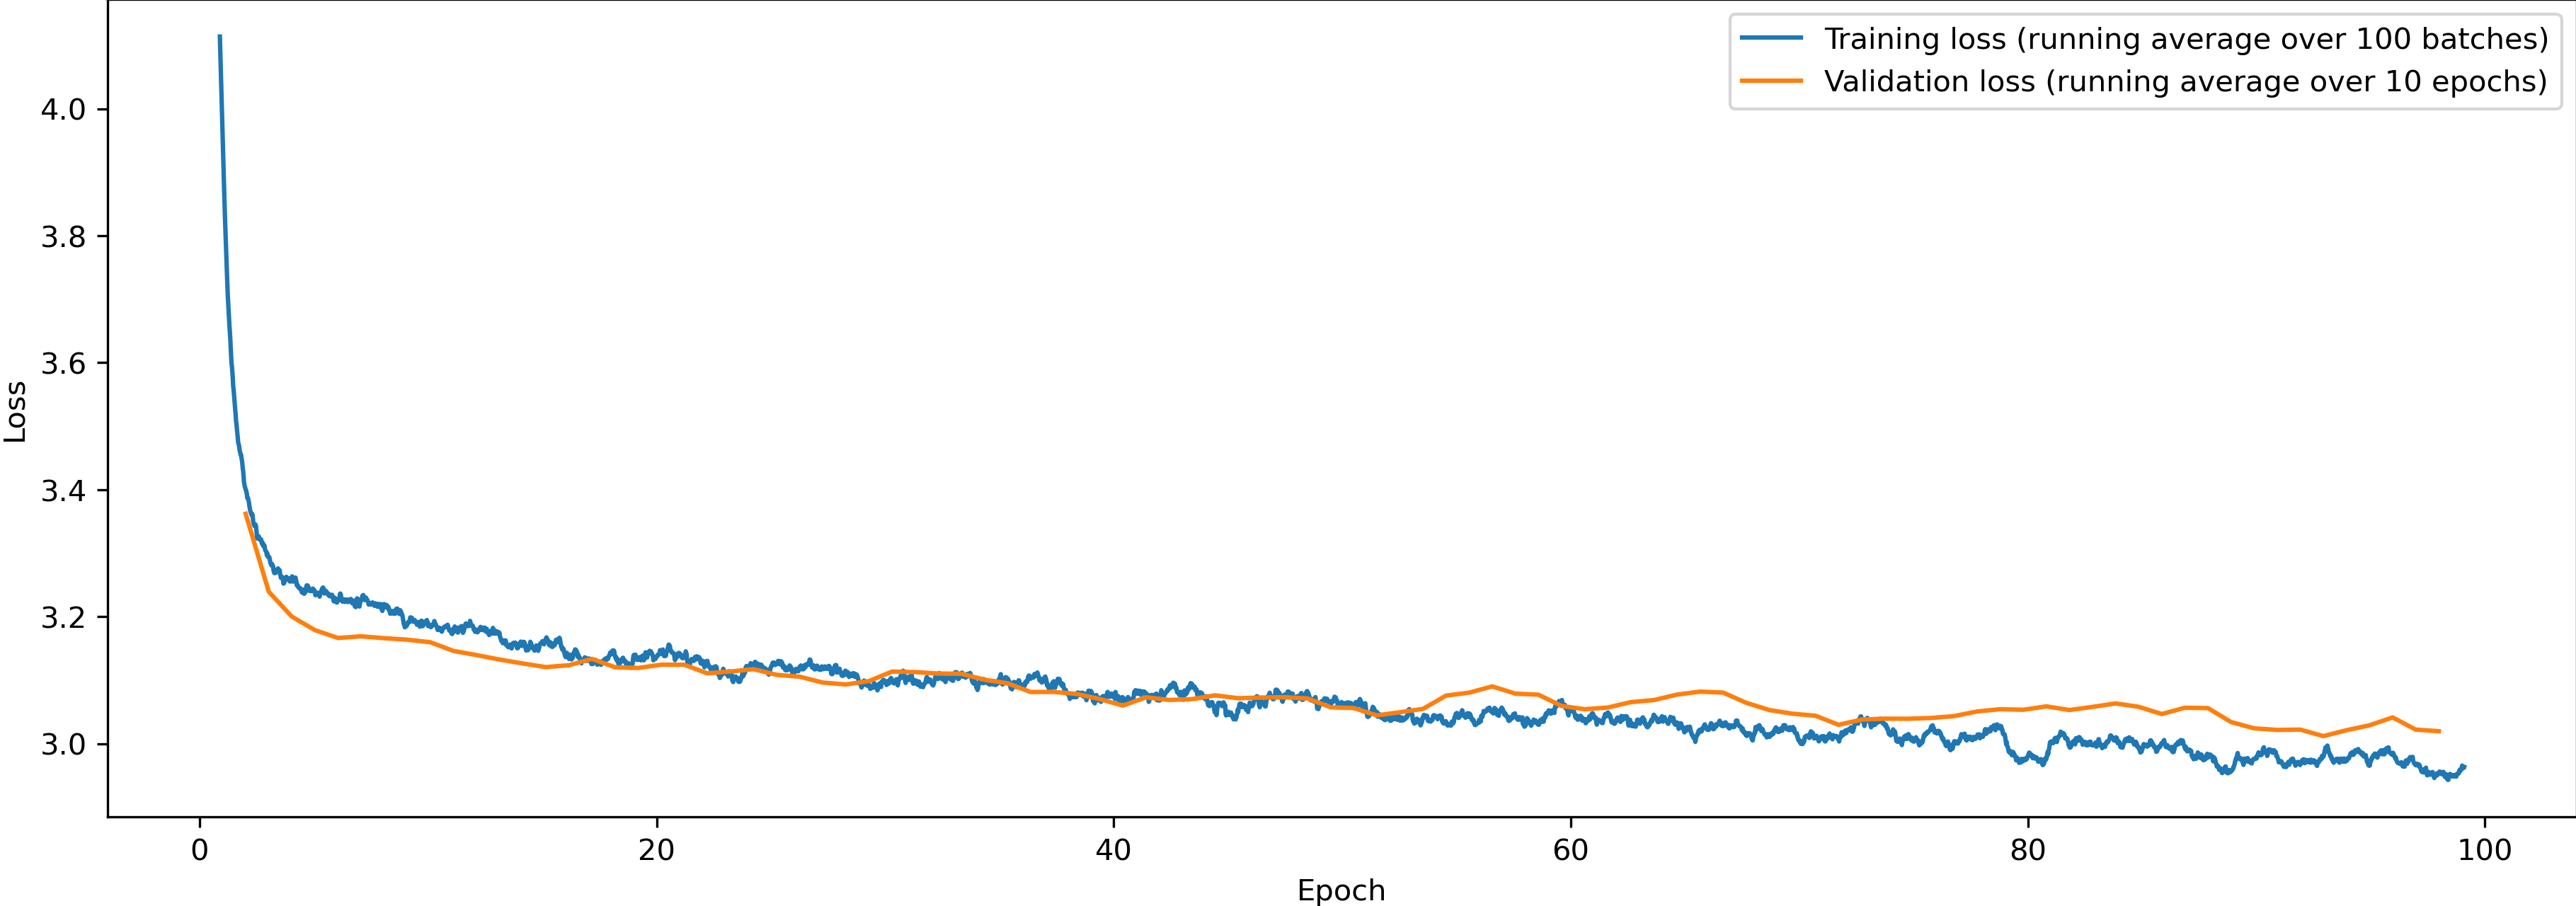
\includegraphics[width=0.75\textwidth]{GRAPHS/unbalanced.png}
        \caption{\textit{Unbalanced} model}
    \end{subfigure}
    \begin{subfigure}[b]{\textwidth}
        \centering
        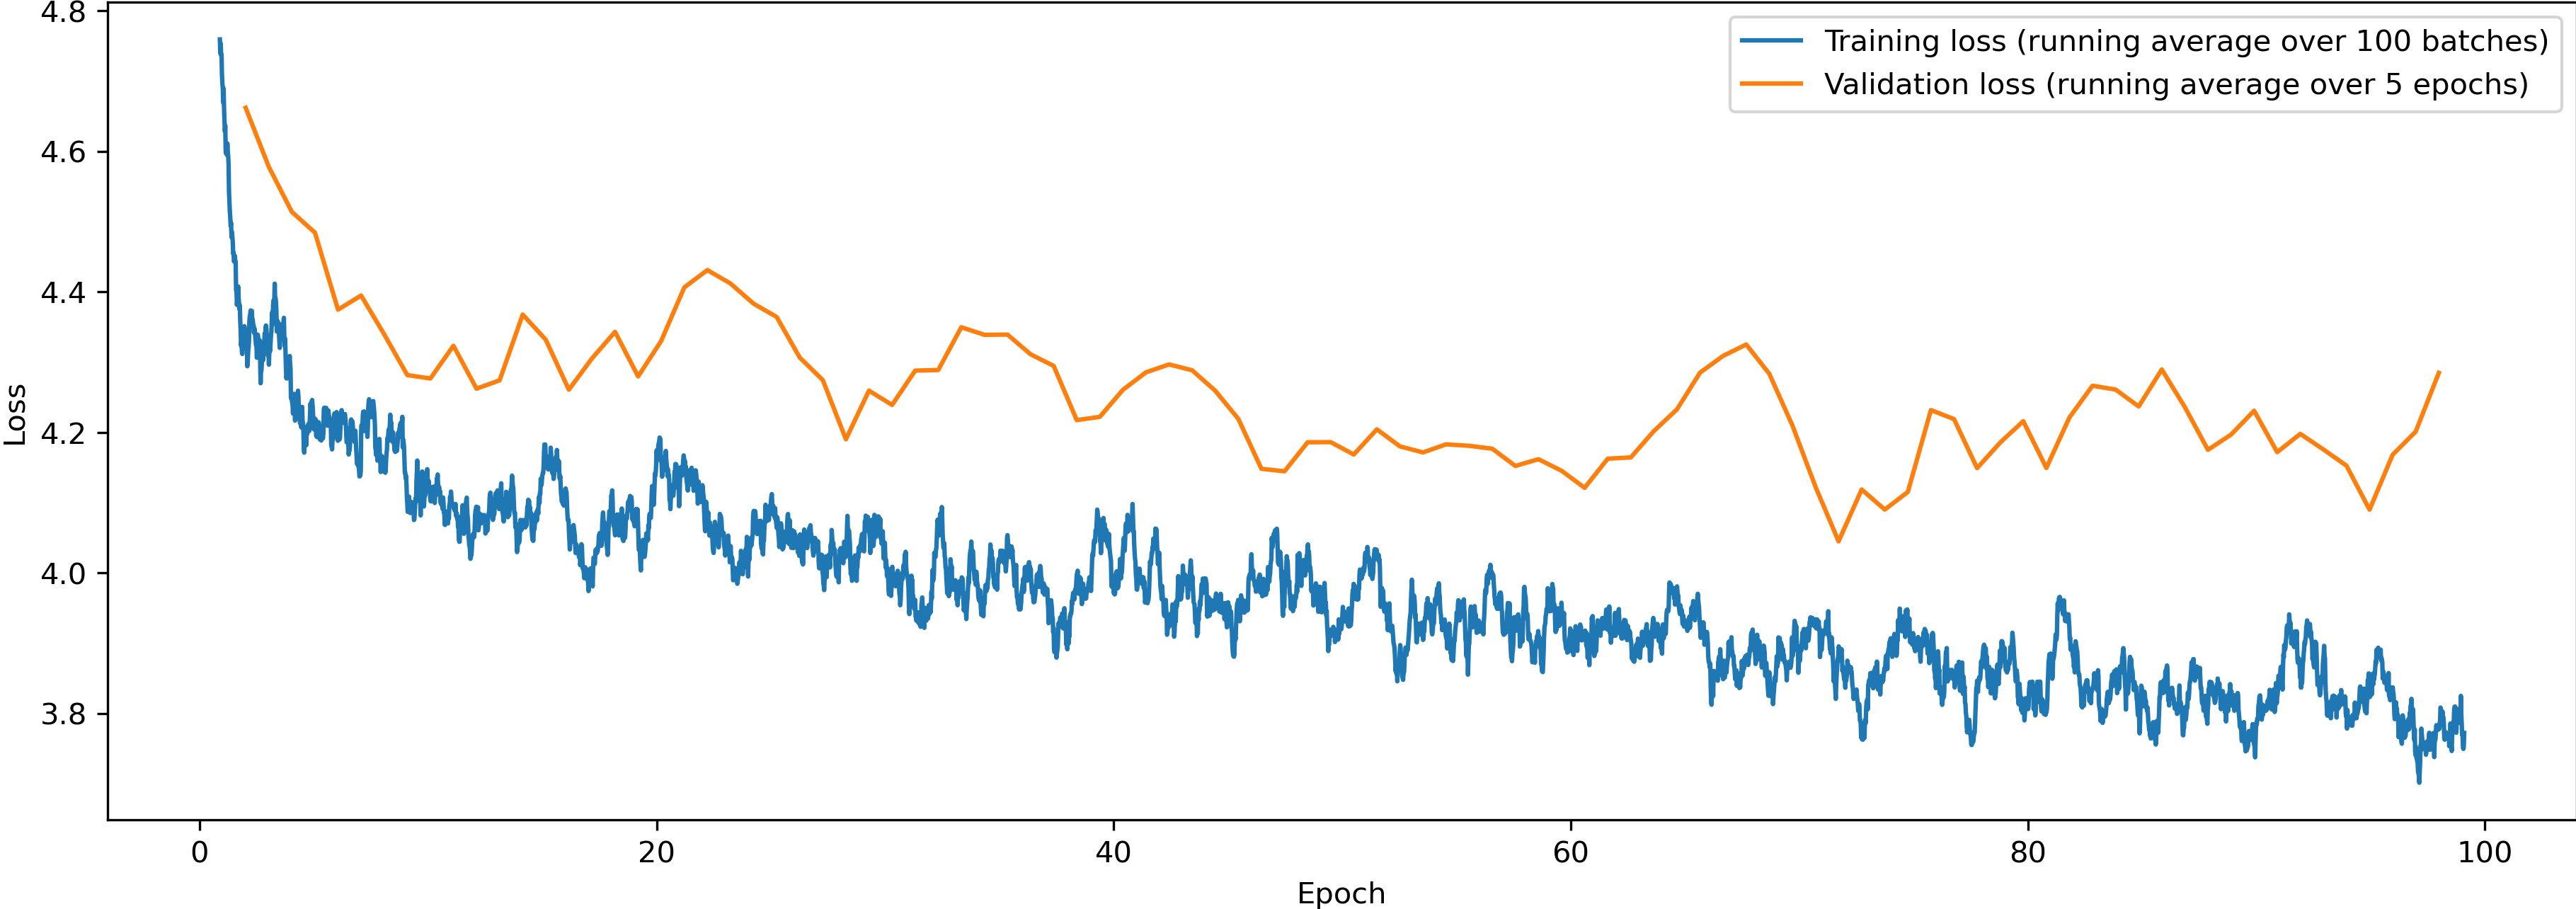
\includegraphics[width=0.75\textwidth]{GRAPHS/rebalanced.png}
        \caption{\textit{Rebalanced} model}
    \end{subfigure}
    \begin{subfigure}[b]{\textwidth}
        \centering
        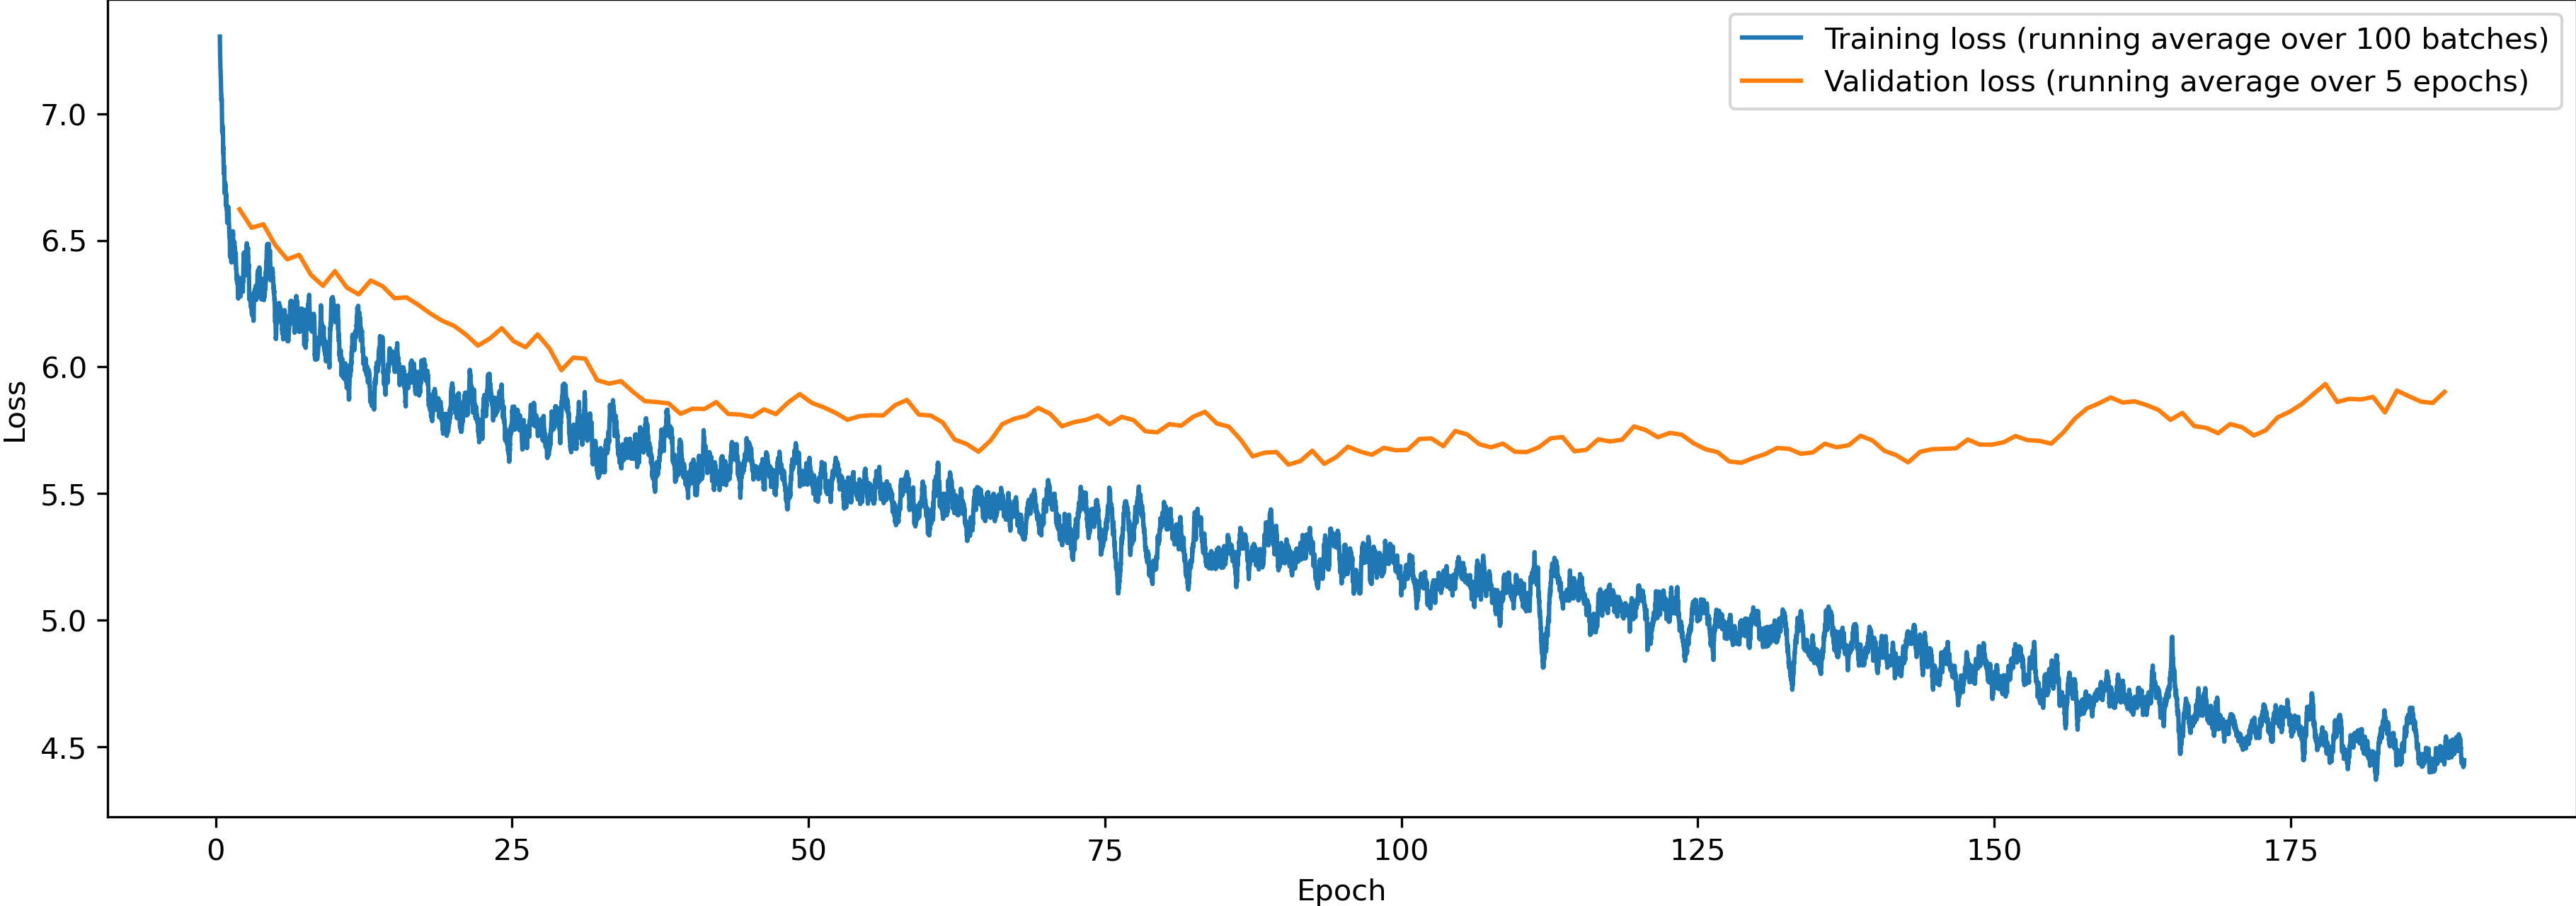
\includegraphics[width=0.75\textwidth]{GRAPHS/rebalanced_ours_final.png}
        \caption{\textit{Rebalanced ours final} model}
    \end{subfigure}
    \begin{subfigure}[b]{\textwidth}
        \centering
        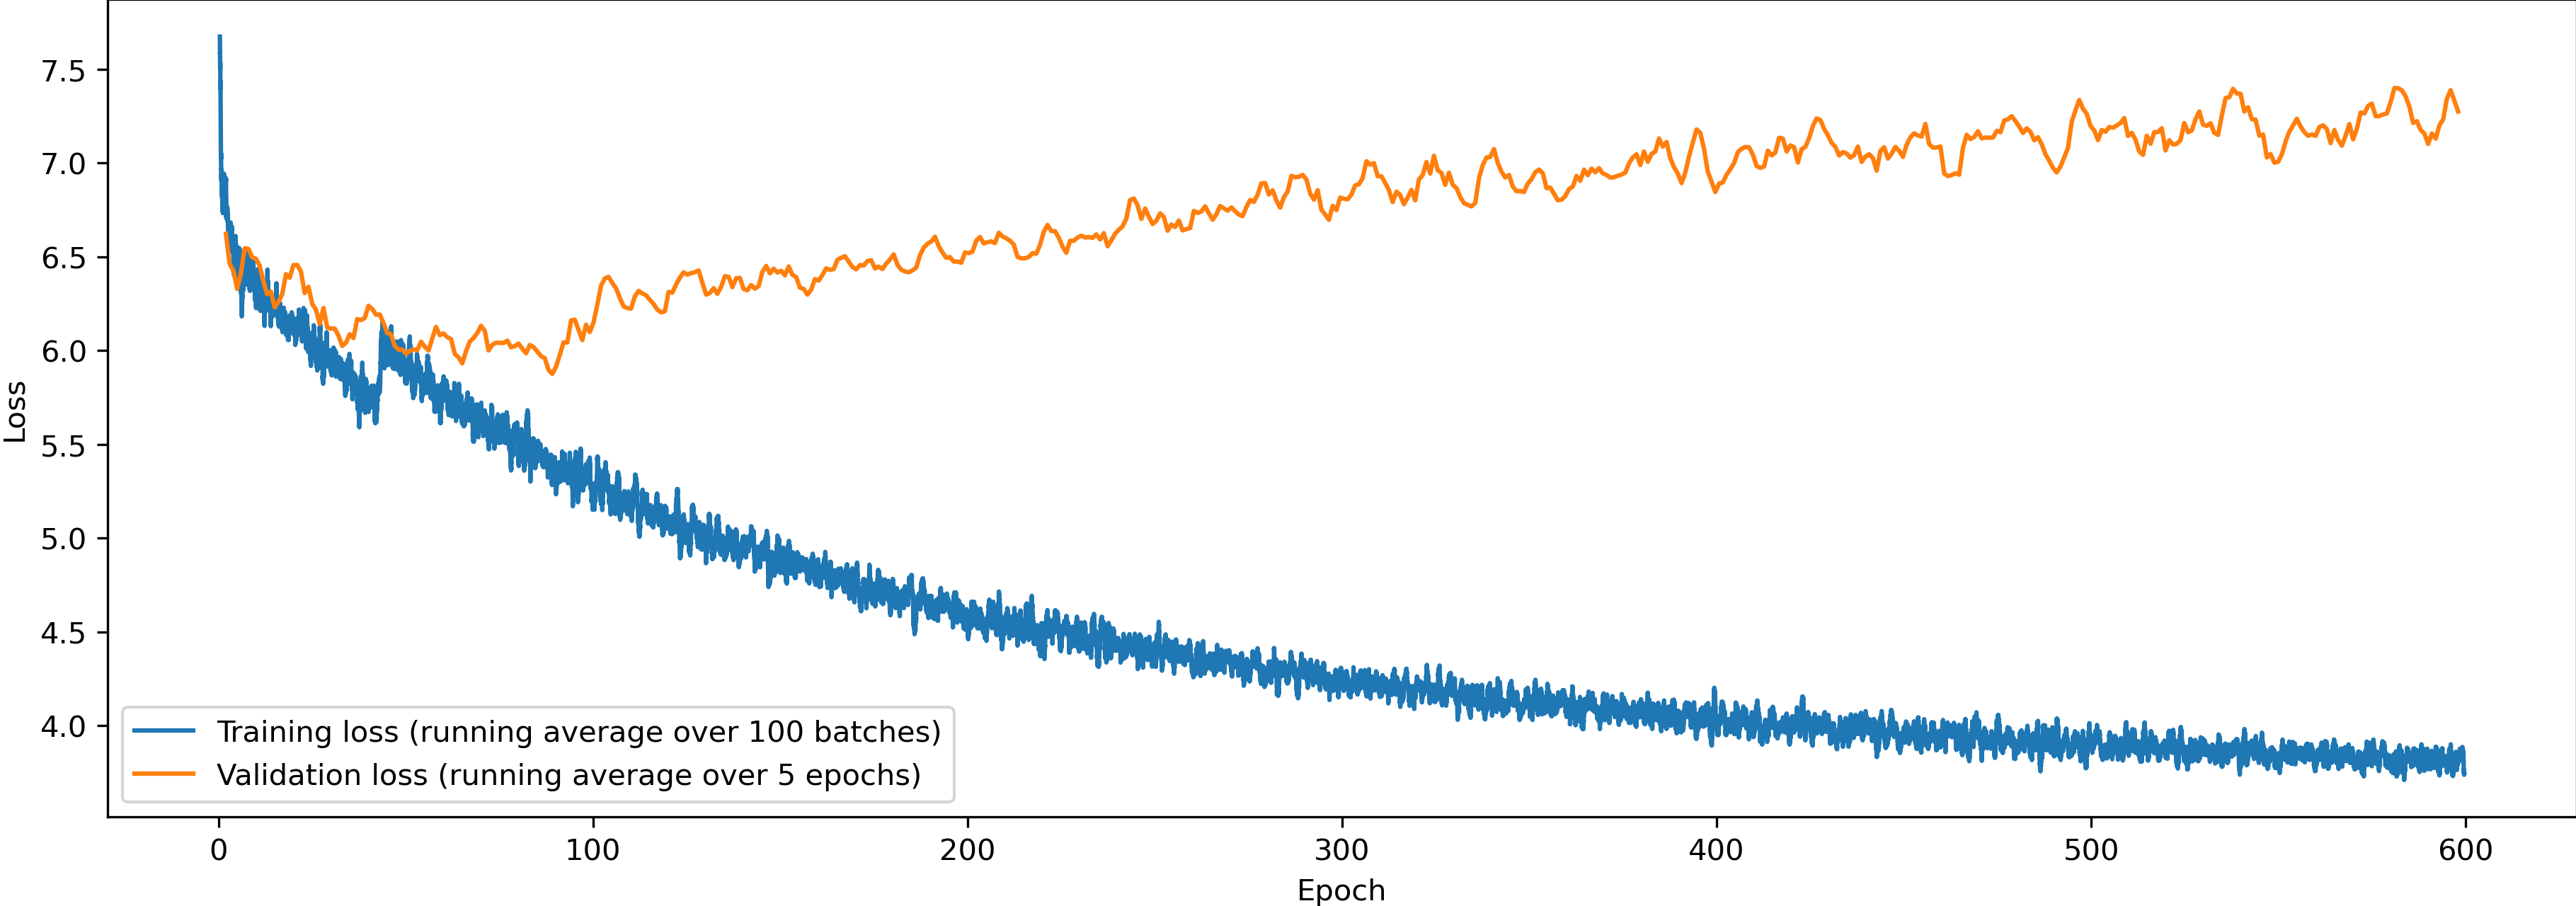
\includegraphics[width=0.75\textwidth]{GRAPHS/simplified_final.png}
        \caption{\textit{Simplified final} model}
    \end{subfigure}
    \caption{Comparison of the learning curves}
    \label{fig:learning_curves}
\end{figure}

\subsection{Evaluation}
Although only subjective human evaluation can truly judge the quality of the predicted images,
the evaluation metrics can help us gauge the performance of the models quantitatively.
They already are a better estimate of what we want to measure, the plausibility of an image colourisation,
than the loss function.

Since the original paper bases the evaluation of their model on subjective human evaluation,
the ability of the model to help a classification model and raw accuracy
(which the authors argue is not a good metric for measuring plausibility), it is not easy
to compare the performance of our models to theirs.\\
Following the advice of the teaching assistants, we decided to use different, automated
evaluation metrics to compare the performance of our models between themselves and to the
baseline model. The metrics we employ are:
\begin{itemize}
    \item \textbf{Root Mean Squared Error (RMSE AB)} calculated over the $a$ and $b$ channels of the true and predicted images;
          note that, since the \textit{Euclidean} model uses this as a loss function, it could naturally have a lower error.
    \item \textbf{Root Mean Squared Error (RMSE)} calculated over the $R$, $G$ and $B$ channels of the true and predicted images;
          the same applies here as for the RMSE AB.
    \item \textbf{Peak Signal-to-Noise Ratio (PSNR)} calculated over the $R$, $G$ and $B$ channels of the true and predicted images;
          it measures the difference between the true and predicted images in decibels and is often used as an approximation of
          the human visual system's perception of reconstruction quality.
    \item \textbf{Structural Similarity Index (SSIM)} calculated over the $R$, $G$ and $B$ channels of the true and predicted images;
          SSIM tries to measure the human perception of image quality by measuring the perceived change in structure
          between the true and predicted images.
\end{itemize}

In Figure~\ref{fig:metrics} we see the results of the evaluation metrics on the testing data across all 9 trained models.
The final models are evaluated on the testing data of the \textit{final} dataset to not bias the evaluation, although if
we evaluate them on the \textit{experimental} subset of the testing data, they perform even better.
Evaluating the models on their respective training and validation data resulted in very similar but slightly better scores.\\
Unsurpisingly, we observe a very close correlation between the RMSE AB and RMSE metrics as they are the same metric calculated
on a different colour space.
Naturally, the \textit{Euclidean} model performs very well here, but the unbalanced models manage to achieve even
lower errors, indicating that they are likely to predict desaturated colours as well.
The models with a rebalanced loss perform significantly worse here, with the \textit{Rebalanced smoothed} model having the highest error.
Of all the models with rebalancing, the \textit{Simplified} models perform the best by far and the
\textit{Simplified final} model even manages to outperform the \textit{Euclidean} model.\\
Turning to the PSNR and SSIM metrics, the difference between the models becomes more subtle.
Again the \textit{Euclidean} and unbalanced models perform well, certainly on PSNR, although
their predictions are not plausible or realistic.
\textit{Rebalanced smoothed} performs again the worst, followed by the \textit{Rebalanced} model.
Using a frequency distribution specific to images of vehicles seems to help, as the
\textit{Rebalanced ours} model scores better on both metrics.
Again, the \textit{Simplified final} model performs best overall due to its long training time, even though it was trained on a wider variety of image classes.
As mentioned before, this is not indicated at all by its validation loss.

\begin{figure}
    \centering
    \begin{subfigure}[b]{0.50\textwidth}
        \centering
        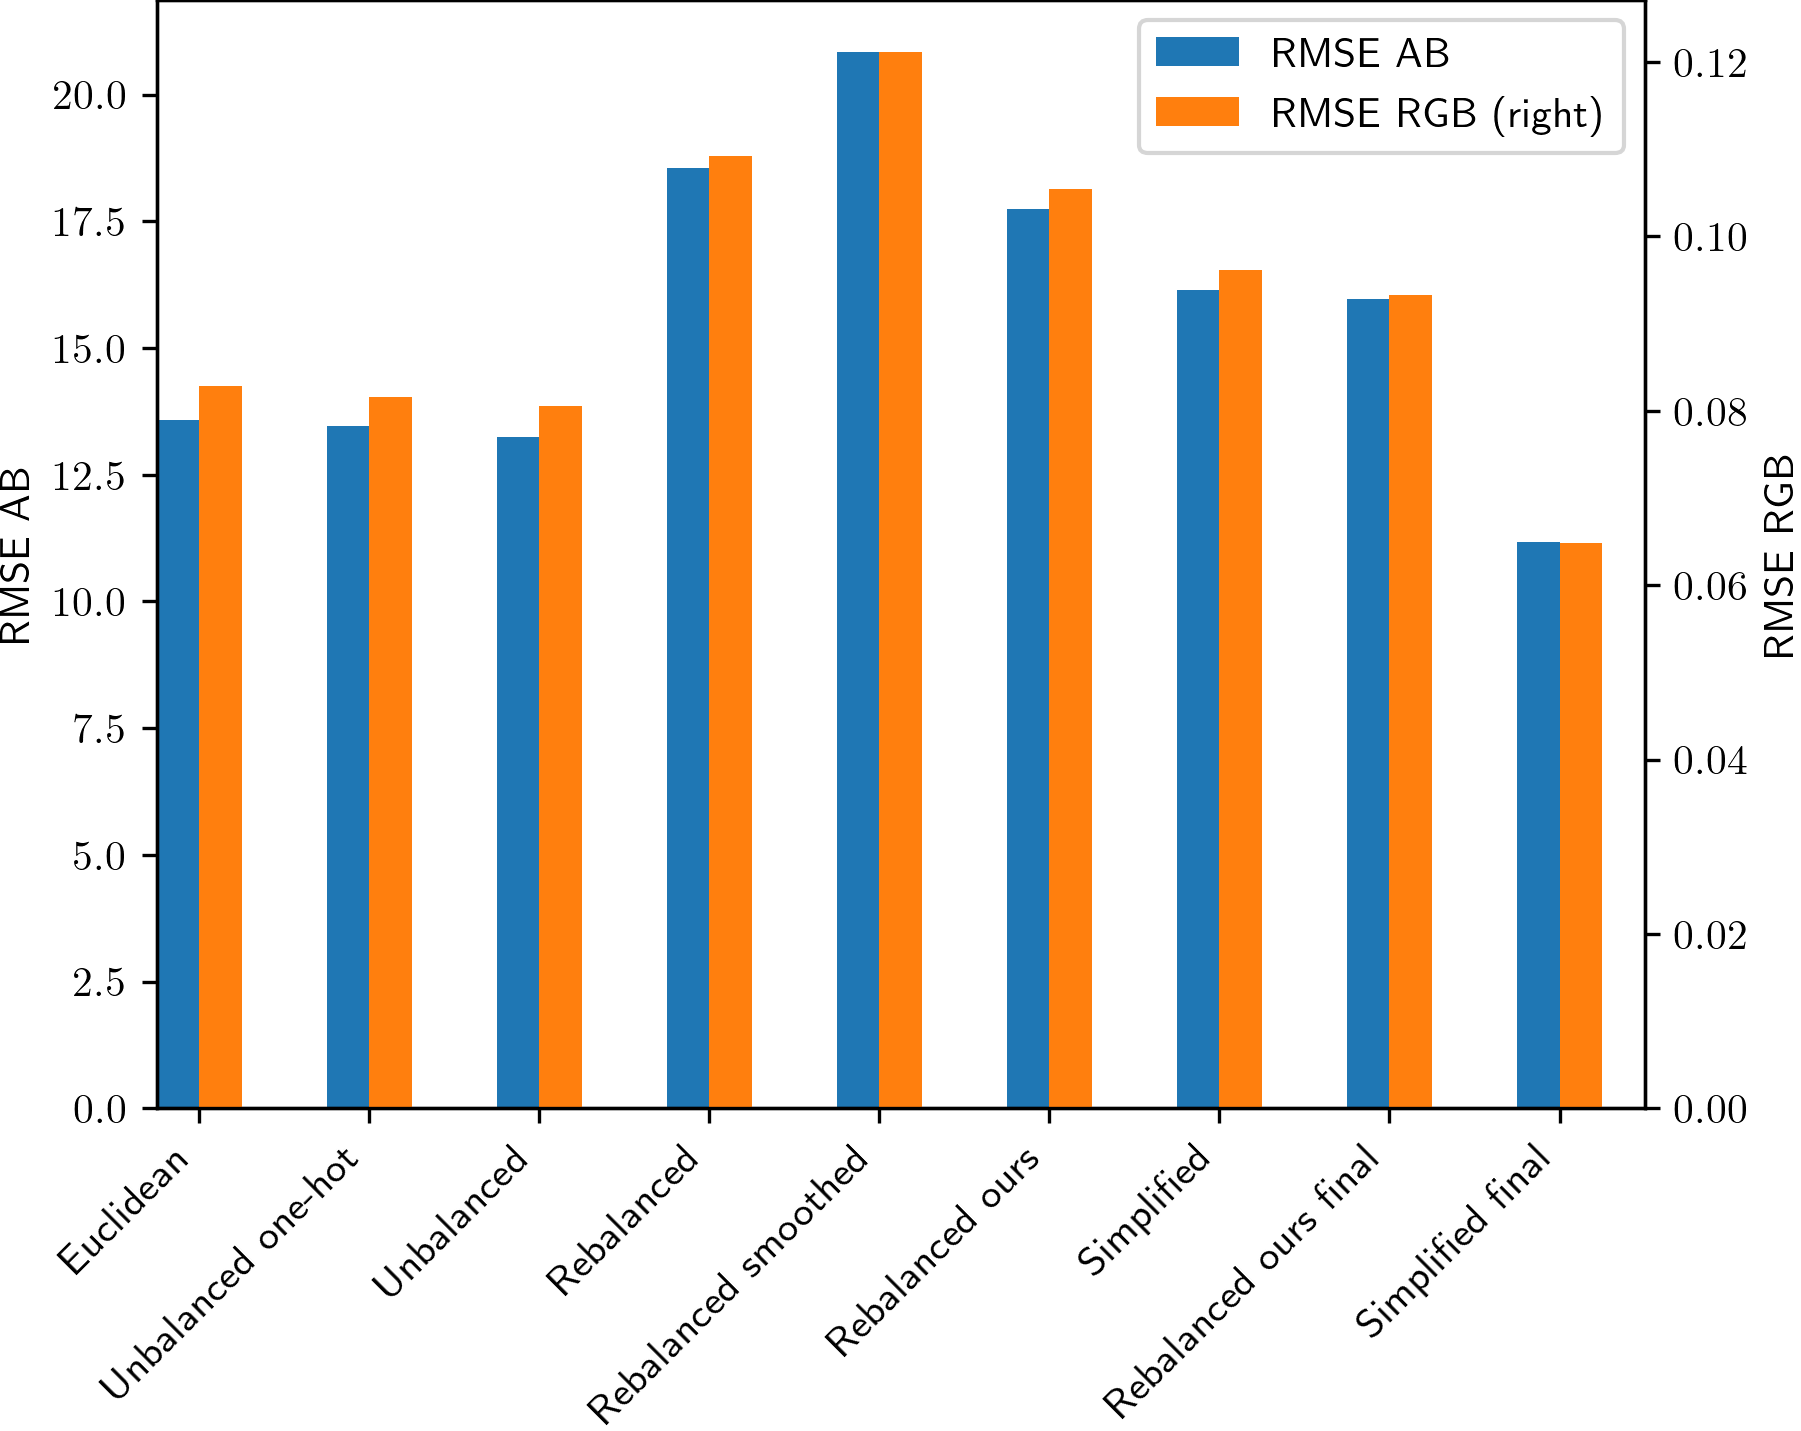
\includegraphics[width=\textwidth]{GRAPHS/rmse.png}
        \caption{Lower is better}
    \end{subfigure}
    \begin{subfigure}[b]{0.48\textwidth}
        \centering
        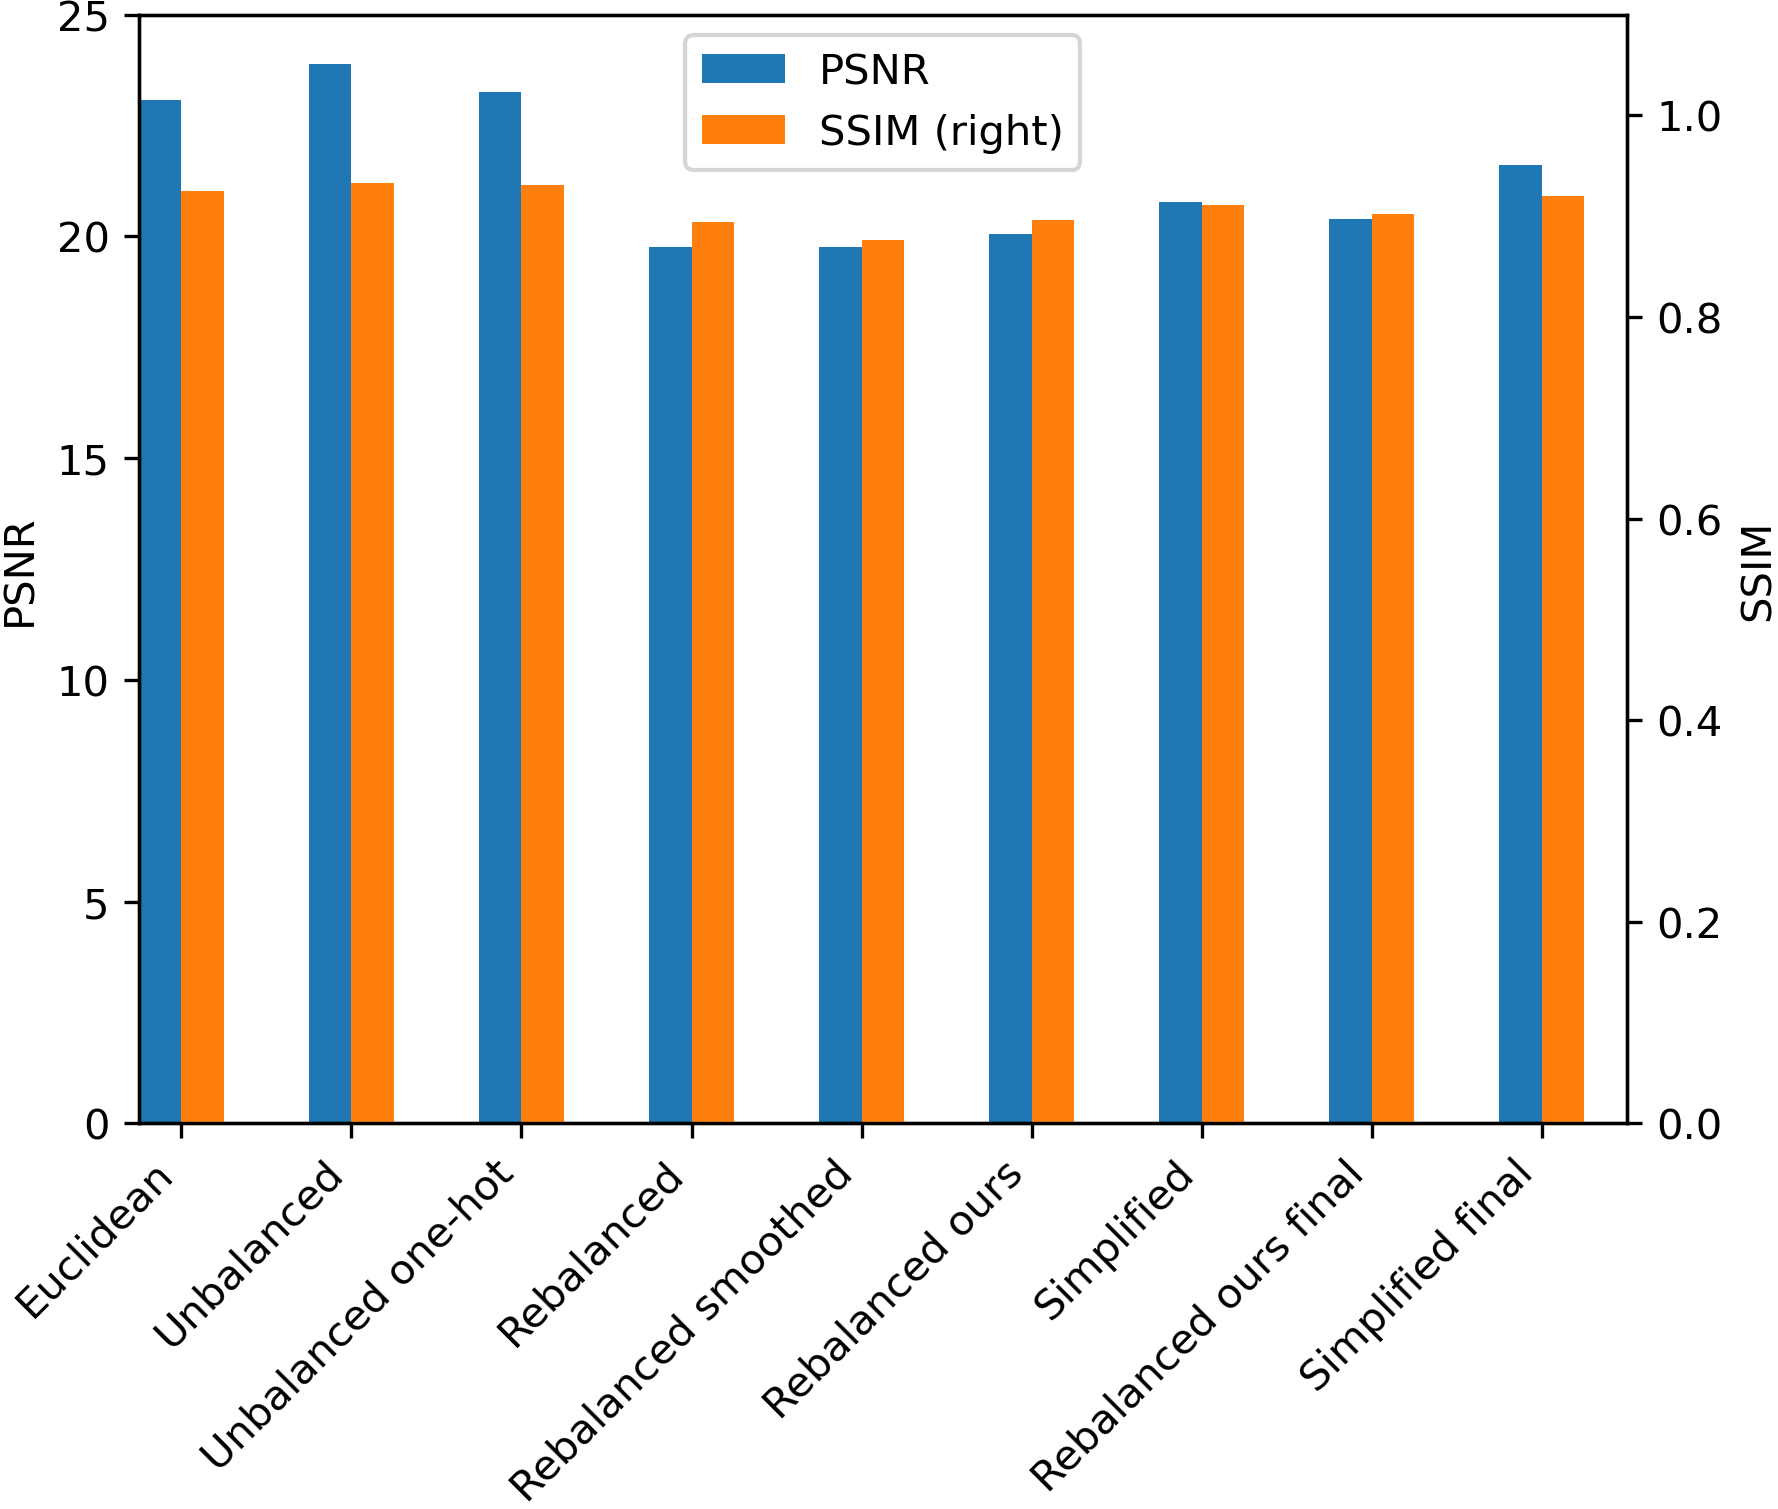
\includegraphics[width=\textwidth]{GRAPHS/psnr_ssim.png}
        \caption{Higher is better}
    \end{subfigure}
    \caption{Comparison of the evaluation metrics on the respective testing data across all 9 trained models}
    \label{fig:metrics}
\end{figure}

\subsection{Experimental Results}
We will now try to characterise the performance of the models in a more subjective way
by visualising some predictions indicative of general trends we observed during the experiments, and
linking this to the evaluation metrics.

We have not yet touched on the effect of the temperature parameter in the annealed-softmax
function used to derive point estimates from the predicted distributions over the colour space.
This is because the temperature parameter does not influence the training of the model,
and can be adjusted even after training to subtly change the predictions.
\cite{colourful} found that a temperature of 0.38 gave the best results, and since this
value also seemed to work well for our predictions in general, we have used it for all the models.\\
In Figure~\ref{fig:temperature} we can see the influence of temperature on the predictions of the \textit{Rebalanced} model,
for which the effect is most pronounced.
The temperature interpolates between the mean colour value of the predicted distribution for a pixel,
resulting in very spatially consistent but desaturated colours, and the mode of the distribution, resulting
in very vibrant but spatially inconsistent colours.
We see this in the figure as increasing the temperature parameter smoothens the borders between the overly saturated colour patches
present in the images to the right, but results in very bland sepia images without colour contrast.
By lowering the temperature,
the annealed softmax distribution becomes more peaked until we obtain the original one-hot encoded distribution,
while increasing the temperature leaves the distribution unchanged.
Intermediate values result in a balance between the two extremes.\\
The influence of the temperature parameter on the predictions of our other models with rebalancing, based on
the dataset-specific colour distribution, is much less pronounced.
We explain this by the fact that the difference in weights used to prioritise the loss for uncommon true colours in our dataset
are already much more contrastive and unsmooth than the ones based on the colour distribution in the entire ImageNet dataset.
This causes the annealed softmax distribution to be very peaked already and decreasing the temperature does not have a large effect on the predictions.

\begin{figure}
    \centering
    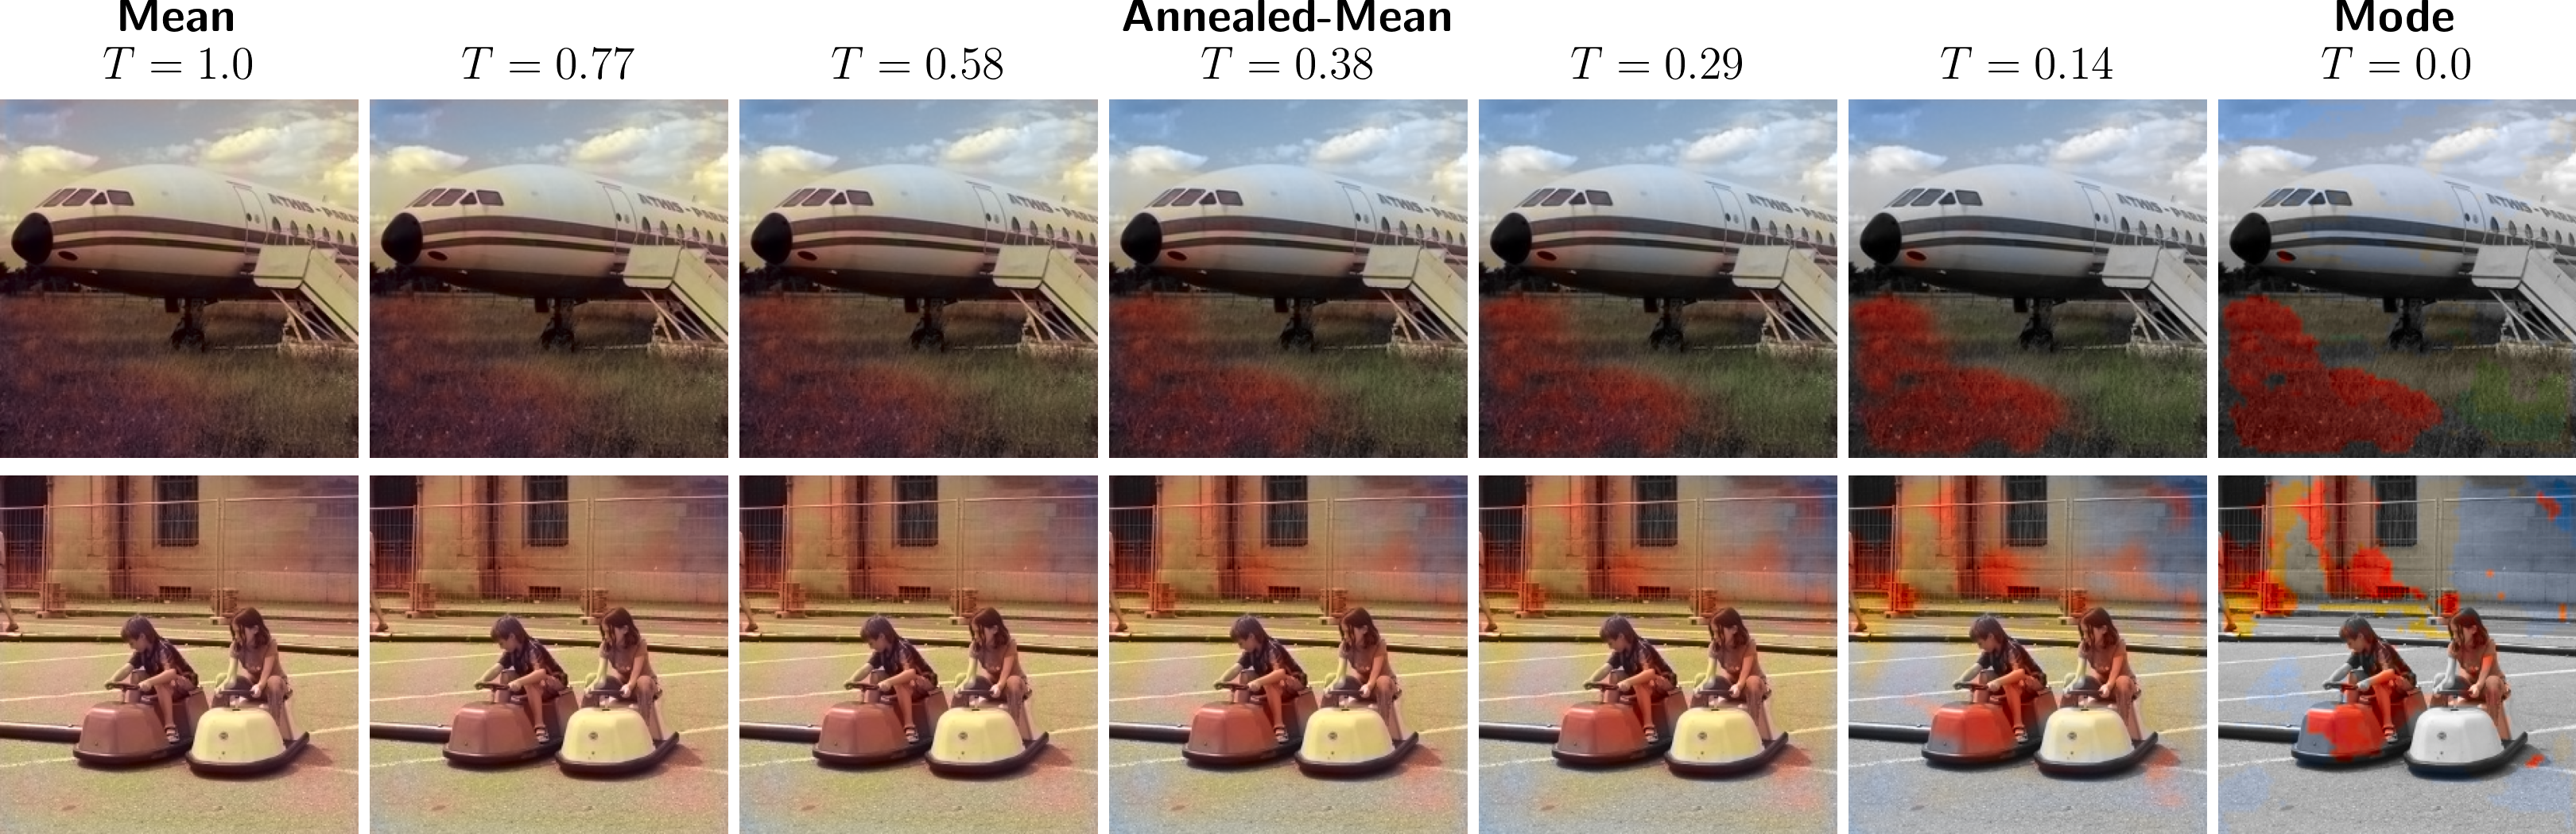
\includegraphics[width=\textwidth]{GRAPHS/temperature.png}
    \caption{The effect of temperature on the annealed-mean output on testing data of the \textit{Rebalanced} model}
    \label{fig:temperature}
\end{figure}

Figure~\ref{fig:comparison} gives a visual comparison of the predictions for 5 testing images, one for each class
in the \textit{Experimental} dataset, across all 9 trained models in chronological order.\\
As expected, the \textit{Euclidean} model is barely able to predict any colour, despite its
evaluation metrics being among the best.\\
The \textit{Unbalanced one-hot} model improves slightly by daring to predict some faint blue colour for the sky
but still fails to predict any other colour in the background or foreground.\\
As hypothesised, using a soft-encoding helps the model in trying to understand the relationship between
the $Q$-values and this can be seen by the appearance of some slightly more nuanced colours in the predictions
of the \textit{Unbalanced} model for grass.\\
The predictions of the \textit{Rebalanced} model indicate some general trends across all models very well.
Most models successfully predict the colour of the sky, grass, water and inside backgrounds since
these often take up a substantial part of the image and are textured very distinctively.
But as seen in the prediction for the image of the boat, they do dare to mix these backgrounds up and,
for example, mistake water for grass.
Because the foreground of the images is often much more detailed, textured and unique, the worse models
fail to distinguish them from the background like in the bumper car image.\\
In contrast to the results of \cite{colourful}, we see that smoothing the weights of the loss function
makes the predictions of the \textit{Rebalanced smoothed} model much worse.
This modification makes the general bias of almost all rebalanced models towards predicting
overly red and saturated patches even more explicit. This explains also the
noticeably worse evaluation metrics of this model.
We contribute this fondness for the colour red to the fact that our dataset barely contains any red objects,
resulting in the reddish colours obtaining a very high weight. As a result, the model tries to predict some probability of red for every pixel it can justify.
This is probably not helped by the fact that images of the
bumper car class, which take up a substantial part of the dataset, are often distinctively hazy and red or pinkish with
very hectic backgrounds (no such images are ever shown in the original paper).
Smoothing the weights makes this only more noticeable by distributing this high bias for red among
all related reddish colours.\\
As indicated by the metrics, the \textit{Rebalanced ours} model improves a bit further on the \textit{Rebalanced} model
by making the colour weights more relevant to vehicle colourisation and, surprisingly, even removing some
oversaturated prediction patches.\\
Although the \textit{Simplified} model has only half the number of parameters, it is by far not inferior to
its bigger brother \textit{Rebalanced ours} for a smaller dataset. This gives the advantage of being able to reduce the
rebalanced loss faster and more consistently and prevents it from overfitting the colour red that much.
Its realistic green prediction for the red car is also a good illustration of what the discrepancy is between
predicting plausible and exact colours. Neither the proposed losses nor metrics can account for this.\\
Finally, at the bottom of the figure, we see the prediction of the final models.
As confirmed by the evaluation metrics, increasing the dataset size and the number of training epochs clearly
benefits the plausibility of the predictions.
The \textit{Rebalanced ours final} model can perfectly distinguish between backgrounds and dares even to
predict unusual, saturated colours in them. Foreground objects do not get confused with the background anymore
but are still too red and hazy to be realistic.\\
The \textit{Simplified final} model takes the crown and predicts surprisingly realistic saturated colours.
It can isolate foreground objects very accurately and makes them pop out.
Training for 600 epochs on a larger dataset has reduced the bias to the colour red to a minimum, sometimes even too much.
Even though this model overfits according to the validation loss, the metrics and predictions show
that it can still generalise well to generate plausible colourisations for new vehicle images.

\newgeometry{left=0cm,bottom=0cm,top=0.4cm,right=0cm}
\begin{figure}
    \centering
    \includegraphics[width=0.6\textwidth]{GRAPHS/comparison.png}
    \caption{Comparison of predictions for 5 testing images from different classes across all 9 trained models}
    \label{fig:comparison}
\end{figure}
\restoregeometry

\section{Conclusion}
While the task of colourising greyscale images is very nuanced and subjective,
we have succeeded in reproducing the results of \cite{colourful} and investigated their claims in detail.
We build on their work by reducing the scope of the task at hand to vehicle colourisation and
propose a simplified network architecture and rebalanced loss function that can be trained on a much smaller dataset.
Using our resources to the limit, we have trained, evaluated and compared 9 different colourisation models,
7 experimental and 2 final.
The resulting \textit{Simplified final} model can generate realistic, plausible colourisations for images of a wide range
of vehicles and outperforms our initial expectations.\\
In investigating the influence of the different components of the models on the predictions on new data,
we encountered a fascinating phenomenon that was not touched upon in the original paper.
Given lightness values for pixels, predicting colour is an inherently ambiguous and multimodal problem, to which multiple
answers are plausible. By comparing the predicted colour distribution to the 'real' distribution, derived through soft-encoding the actual colour labels,
we do not measure the actual achievement of the colourisation task, which is to generate \textit{plausible} colourisations.
As such, neither the Euclidean loss, cross-entropy loss, nor the proposed rebalanced loss are perfect loss functions, as they fail
to capture this ambiguity by comparing only against an encoding of the colour label.\\
This discrepancy between the loss function and the task goal explains why overfitting the \textit{Simplified final} model
to the expanded training dataset did not result in worse predictions on new data.
This phenomenon only highlights the importance of creating a loss function that captures the actual goal of the task
as closely as possible, as this is one of the most important components of a successful deep-learning model on which
the designers have the most control and insight.
As a secondary measure, the evaluation metrics can help us gauge the performance of the model quantitatively and
give us a more informed indication of how well a machine learning model performs a task.\\
In this way, even the most subjective and nuanced tasks, assumed to be particular to humans, can be tackled by machine learning.

\bibliography{report}
\bibliographystyle{plain}
\end{document}
